\chapter{测度空间}
\label{chap:measure-spaces}

在前面的微积分里，我们累计一个量时，底集总是实轴或欧氏空间：长度、面积、体积已经替我们规定好“一块区域有多大”，积分就是在这套规定上累计函数。
但在机器学习中，需要累计的对象往往不是数：它们可能是词、类别、图、数据样本，或者另一个空间里的点。
这时长度和体积帮不上忙，我们必须自己回答两件事——哪些集合允许被测量，以及测量的结果是多少。
回答这两个问题的工具，就是\emph{可测结构}和\emph{测度}。

读到这里很容易把“测度”和前一章的“度量（距离）”混为一谈，因为两者都在描述空间的“大小”，名字也只差一个字。
它们其实回答完全不同的问题，最好一开始就分清楚。
\emph{度量}吃进去的是\emph{两个点}，吐出来一个距离$d(x,y)$：它衡量两点隔多远，输入空集或一个集合时没有意义，而且要求$d(x,y)=d(y,x)$、$d(x,x)=0$。
\emph{测度}吃进去的是\emph{一个集合}，吐出来这个集合的“份量”$\mu(A)$：区间给长度、一群点给总权重，但它对“两点之间多远”完全不说话。
一句话对比：度量回答“$x$和$y$离得多近”，测度回答“集合$A$有多重”。
同一个点集上可以先任选一个度量、再任选一个测度，两者互不决定——例如在实轴上，标准距离配上计数测度，或者把常走的两点间距离改小而长度测度不变，都是完全合法的。
本章的“可测空间/测度空间”只需要第一层（集合的份量）；等到讨论Wasserstein距离、开球和紧性时，才在测度之外\emph{另外}加一个度量。

\begin{figure*}[htbp]
\centering
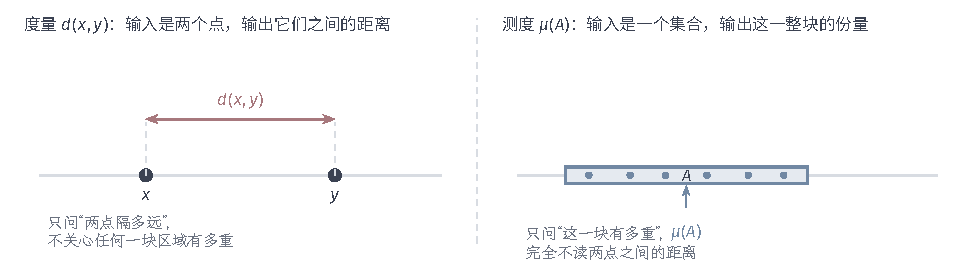
\includegraphics[width=169mm]{figures/01-mathematical-preliminaries-upper/04-space-and-geometry/02-measure-spaces/tikz/measure-vs-metric/figure.pdf}
\caption{度量与测度回答的是两个不同问题。度量$d(x,y)$以两个点为输入，给出它们之间的距离，并要求对称、$d(x,x)=0$、三角不等式；测度$\mu(A)$以一个集合为输入，给出这一整块的份量，并要求空集为零、可数可加。同一底集上度量与测度可以各自独立选择，互不决定。}
\label{fig:measure-vs-metric}
\end{figure*}

先看一个具体场景。
给定一批数据上的两种分布，我们会问：它们是不是一回事？如果不是，差在什么地方？
有时两种分布描述的是同一组对象，只是各部分占的比重不同：比如同一批人按两种口径统计收入。
有时它们根本描述不同空间的对象：比如一张图片和它的类别标签，需要一条规则说明图片上的“质量”怎样传到标签上。
这两类问题构成本章的两条主线。

第一条主线固定同一个空间，只比较上面的两种赋权。
我们要判断一种赋权认为是零的集合，另一种是否也认为是零；能不能找到一个密度函数，用一种赋权把另一种表示出来；以及用一个数概括两者的整体差异时，不同指标各在衡量什么。
第二条主线允许空间不同。
给定一个映射时，输入空间的质量怎样“推”到输出空间；当一个输入不只对应一个确定输出，而是按某种概率分散到若干输出时，这种规则怎样描述；如果还想知道输入与输出是怎样配对的，又要付出什么跨空间的移动代价。

\ref{sec:measure-general-structure}节先打基础，把实轴上已经熟悉的可测集合、测度、积分和乘积推广到一般空间。
\ref{sec:measure-same-space-comparison}节回到第一条主线，比较同一空间上的测度。
\ref{sec:measure-cross-space}节处理第二条主线，研究映射、测度核、联合测度和跨空间运输。
\ref{sec:measure-convergence}节再让测度随序号或时间变化，讨论一列测度怎样才算趋近、在什么条件下一定能找到收敛的子列。

这些内容不是几种互不相干的“测度种类”，而是同一套工具在回答不同问题。
确定映射其实是一种特殊的测度核：它给每个输入指派的输出测度全部集中在一个点上。
全变差、Wasserstein等差异指标也有联系：有的只看同一事件上的质量差，有的还关心两点在空间中隔得多远，我们会在相应位置把关系讲清。
概率测度在本章只是总质量恰好为$1$的测度；条件期望、Bayes公式、随机过程等需要额外概率结构的内容都留给后文，这里只建立可以反复调用的通用对象和运算。

\section{一般测度的结构与积分}
\label{sec:measure-general-structure}

在实轴和欧氏空间上，“一块区域有多大”是由长度、面积、体积直接给出的。
换到一般对象的集合后，这种天然的大小不存在了，我们要自己把测量的规则补回来。
本节做四件准备工作：先说清哪些集合允许被测量、再说明怎样给这些集合配质量；然后引入开集、闭集等拓扑概念在测量中的位置；接着把熟悉的积分搬到一般测度上；最后处理两个空间的联合结构。
这些内容在实轴上都已经出现过，这里不重复证明，重点是看清“换了底集以后，哪些结论原封不动，哪些条件必须重新声明”。

\subsection{可测结构与基本赋权}

拿到一个由任意对象组成的集合后，测量要分两步走，而且两步互不相干。
第一步决定\emph{哪些集合看得见、可以测量}，这是可测结构；第二步决定\emph{看得见的集合各自有多大}，这是测度。
同一套可见集合上可以配完全不同的质量，同一个质量的想法在更粗或更细的可见范围下也要分别讨论。
本小节先建立这两层，再给出点质量、测度混合和零测例外的说法。

\subsubsection{可测范围与子$\sigma$代数}

\paragraph{可测空间与生成结构}

设$X$是我们关心的全部对象，例如若干类别、若干样本或若干状态。
要测量它的子集，先要圈定一个“允许测量的集合族”。
为什么不能直接宣布所有子集都可测？
在实轴上已经看到，一旦允许不可数次地分割、覆盖和取极限，就会出现无法自洽赋长度的集合；因此允许范围必须满足一定封闭性，但又不能大到没有限制。

我们沿用$\sigma$代数的要求：集合族$\mathcal A\subseteq\mathcal P(X)$包含全集$X$，并且对相对补集和可数并封闭。
取补和可数并还自动带来另外几种封闭：空集属于$\mathcal A$，可数交
\[
 \bigcap_nA_n=X\setminus\bigcup_n(X\setminus A_n)
\]
属于$\mathcal A$，两个可测集的差$A\setminus B=A\cap(X\setminus B)$也属于$\mathcal A$。
换句话说，凡是能用可测集合作可数多次集合运算得到的集合，仍然允许测量。
配备了这样一个集合族以后，二元组$(X,\mathcal A)$称为可测空间，$\mathcal A$中的集合称为可测集合。

实际问题里，我们往往只先点名少数几个必须能测量的集合，例如区间、矩形或某些类别，其余集合由它们“生成”。
对一族集合$\mathcal C$，包含它的$\sigma$代数可能有很多，其中最小的一个记为$\sigma(\mathcal C)$。
最小性可以这样理解：幂集$\mathcal P(X)$总是一个包含$\mathcal C$的$\sigma$代数，所有这种$\sigma$代数的交仍然包含$X$且对补集、可数并封闭，所以交出来的最小范围确实存在。
这种“只规定少数起点，再封闭出全部可测集”的做法非常省事：后面验证一个映射是否可测、两项测度是否相同，都只需在起点集合上检查，再由封闭性推广到整个$\sigma$代数。

用一个有限例子体会“可见”的含义。
在$X=\{1,2,3,4\}$上，幂集$\mathcal P(X)$允许区分每一个点；但由划分$\bigl\{\{1,2\},\{3,4\}\bigr\}$生成的$\sigma$代数只有
\[
 \bigl\{\varnothing,\{1,2\},\{3,4\},X\bigr\}.
\]
在这套范围里，“第$1$个点”单独是看不见的，能测量的只有前两个点、后两个点这两个分块。
可见集合的多少，决定了我们能在多大精度上讨论问题。

\paragraph{子$\sigma$代数与同一底集上的粗化}

有时底集不变，但我们主动“眯起眼睛”，只看其中一部分集合。
若$\mathcal G\subseteq\mathcal A$本身也是一个$\sigma$代数，就称它为\term{子σ代数}。
$(X,\mathcal G)$中的对象一个不少，仍是原来的$X$，只是可见的集合变少了。
这种操作叫粗化，它和“把底集缩小成子集$Y\subseteq X$”不同：缩小底集是扔掉一批对象，粗化只是降低对同一批对象的分辨能力。

仍以四点集合为例。
在$\mathcal A=\mathcal P(X)$下四个单点都能单独测量；换成
\[
 \mathcal G=\{\varnothing,\{1,2\},\{3,4\},X\},
\]
就只能称“前两点合起来多重”“后两点合起来多重”，再也无法分开第$1$点和第$2$点。
若原来在$\mathcal A$上有测度$\mu$，只在$\mathcal G$上读取它，记作$\mu|_{\mathcal G}$，这只是缩小赋权规则的定义域，并没有删除任何点。
后面讨论\term{条件积分}时，会专门研究“在只能看到$\mathcal G$的情况下，怎样保留各分块上的累计信息”；这里先把粗化这种结构本身建立起来。

\subsubsection{测度、混合与零测例外}

\paragraph{一般测度及有限性条件}

圈定可见集合以后，就要给每个集合配一个非负的“大小”。
设$\mu$把每个可测集映到$[0,+\infty]$。
要求它满足两条：空集的大小为$0$；把互不相交的可数个集合合并时，总大小等于各部分大小之和，即
\[
 \mu\!\left(\bigcup_{n=1}^{\infty}A_n\right)=\sum_{n=1}^{\infty}\mu(A_n).
\]
这样的$\mu$称为测度，$(X,\mathcal A,\mu)$称为测度空间。
第二条（可数可加）是测量的核心：它保证“分成几块分别称，再合起来称”，结果一致。
底集换成一般对象后，这个直觉与长度完全相同；由它还能立刻得到单调性$A\subseteq B\Rightarrow\mu(A)\leq\mu(B)$和可数次可加，证明与实轴上一样，不再重复。

后面的定理对“总质量有多大”有不同要求，这里先把三个常用名词一次分清，免得以后混淆。
若$\mu(X)<\infty$，称$\mu$为\term{有限测度}；进一步若$\mu(X)=1$，称$\mu$为\term{概率测度}，此时每个集合的质量都在$[0,1]$内。
还有一个更弱、却非常常用的条件叫$\sigma$有限，满足它的测度即\term{σ有限测度}：可以用可数个可测集$E_k$盖住$X$，使每一块的质量都有限。
三者关系是：概率测度一定有限，有限测度一定$\sigma$有限（取$E_1=X$），但反过来不成立。
自然数集上的计数测度给每个点质量$1$、全空间质量无穷，却能被单点集$\{1\},\ldots,\{k\}$有限地盖住；实轴上的勒贝格测度总质量无穷，但区间$[-k,k]$每一块都有限——它们都是$\sigma$有限而不有限。

集合列的连续性沿用前面的结论，但要留意有限性出现在哪里。
集合逐渐扩大时，$A_n\uparrow A$就有$\mu(A_n)\uparrow\mu(A)$，不要求任何有限性；集合逐渐缩小时，$A_n\downarrow A$要得到$\mu(A_n)\downarrow\mu(A)$，必须先有$\mu(A_1)<\infty$。
否则$(n,\infty)\downarrow\varnothing$，而每一项的勒贝格长度都是无穷，无法相减得到零。
请记住：$\sigma$有限不是所有运算的万能前提，密度表示、乘积构造和有界函数积分各自需要的条件，会在用到时分别说明。

\paragraph{加权点测度与\term{可数混合}}

最容易想象的测度，是把质量直接放在若干个点上。
固定一个点$x$（并假设$\{x\}$可测），定义
\[
 \delta_x(A)=\mathbf 1_A(x)=
 \begin{cases}1,&x\in A,\\0,&x\notin A,\end{cases}
\]
称为集中在$x$的点质量：集合包含$x$就得质量$1$，否则得$0$。
它对应“全部重量压在一个点上”的极端赋权。

再取一列点$x_i$和非负权重$w_i\geq0$，把若干点质量加起来：
\[
 \mu=\sum_i w_i\delta_{x_i},\qquad
 \mu(A)=\sum_i w_i\,\mathbf 1_A(x_i).
\]
因为每个点属于哪些不交集合是唯一确定的，两个非负求和可以交换次序，所以$\mu$仍然可数可加；同一位置上的权重自动相加。
权重总和有限时$\mu$是有限测度，总和为$1$时就是概率测度。
这里有个细节：定义本身不要求每个单点都可测，但只要具体计算中用到$\delta_x(\{x\})=1$，就必须先确认$\{x\}\in\mathcal A$。

同样的“加权相加”还可以用在测度上。
设$\mu_i$是同一空间上的非负测度，取非负系数$a_i$，令
\[
 \mu(A)=\sum_i a_i\mu_i(A),
\]
非负级数换序保证$\mu$仍是测度。
若各$\mu_i$都是概率测度且系数和为$1$，得到的就是可数混合：以比例$a_i$在第$i$种随机规律之间随机挑选一种。
一个直观例子是
\[
 \mu=\tfrac12\,\lambda|_{[0,1]}+\tfrac12\delta_0:
\]
一半重量像水一样均匀铺在$[0,1]$上按长度分配，另一半重量全部压在点$0$上。
这样的混合提醒我们：一个测度完全可以同时拥有“连续铺开”的部分和“集中成点”的部分。

\paragraph{零测例外与完备化}

测量时，质量为零的集合允许我们忽略其中点上的例外。
可测集$N$若满足$\mu(N)=0$，称为零测集；某性质$\mu$几乎处处成立，是指不满足性质的点全部能装进某个可测零测集。
但“可以忽略”永远是相对于具体测度而言的：在勒贝格测度下单点$\{0\}$质量为零，可以忽略；在$\delta_0$下它的质量却是$1$，恰好是唯一重要的点。
还要注意例外能够合并的规模：可数个零测集的并仍是零测集，所以可数多个“几乎处处成立”的结论可以共用一个例外范围；不可数个零测集的并则没有这种保证。

另一个相关的性质是完备性。
若每个可测零集的任意子集都仍然可测，就称这个测度空间完备。
不完备时，可能有一个集合包含在零测集里，它本身却不可测——我们知道它“应当质量为零”，却无法在规则内给它赋值。
补救办法是完备化：把这些缺失的零测子集、以及它们与原可测集的并全部补进可测范围，并按外面的零包络赋零。
补进去以后，原来集合的测量值一个都不变，只是可测范围成为满足要求的最小扩展。
实轴上的具体构造前一章已经做过，这里只需理解它的作用：有了完备化，在零测集上随意改动一个函数的值，得到的函数仍然可测；否则“几乎处处相同”的两个函数可能一个可测、一个不可测。
因此使用几乎处处等价的函数时，要么挑一个可测的代表来用，要么明确进入完备化空间，不能简单地以为“反正是零测，怎样都行”。

\subsection{测度与拓扑结构}

仅有可测结构时，我们知道一个集合能否测量，却说不清它是开是闭、是远是近。
后面比较测度时，有些指标（例如全变差）完全不需要位置信息，另一些指标（例如Wasserstein）则必须知道两点之间的距离。
本小节把这两类条件分开：先说明开集怎样进入可测结构，再定义“测度集中在哪里”的\term{支持}。

\subsubsection{Borel结构与标准Borel范围}

\paragraph{从开集生成Borel结构}

当$X$本身带有拓扑（从而能谈开集、闭集）时，最自然的可测范围是让所有开集都可测，再封闭出其余集合。
这个由全体开集生成的$\sigma$代数称为Borel结构：
\[
 \mathcal B(X)=\sigma(\{U\subseteq X:U\text{ 是开集}\}).
\]
于是开集、闭集以及对它们作可数并、可数交、取补得到的集合都可测。
在实轴上，开区间都是开集，这个定义与前一章“由开区间生成$\mathcal B(\mathbb R)$”完全一致。
在离散空间里每个单点本身就是开集，所以Borel结构等于幂集；实轴的Borel结构却不等于全部子集，不可测集依然存在。
请特别注意：选定Borel结构只决定了“哪些集合可测”，它本身\emph{没有指定任何测度}；同一个$\mathcal B(\mathbb R)$上既可以放长度，也可以放正态分布或一个点质量。

选定一个\term{Borel测度}后再做完备化，可测范围还可能扩大。
例如勒贝格可测集族$=$实轴Borel集族$+$所有勒贝格零集的子集，比Borel结构更大。
因此要分清三个层次：拓扑规定开集，Borel$\sigma$代数由开集生成，完备化还要依赖具体选了哪个测度。
后文说“在标准Borel空间上成立”时，指的是中间这一层；不能不加核对地把完备化后才出现的集合代进去。

\paragraph{\term{Polish空间}与\term{标准Borel空间}}

后面的距离比较和测度分解经常需要一个“足够规整、又足够常见”的舞台，为此引入两个条件。
一个拓扑空间若既能找到可数个点稠密地铺在其中（可分，因而开集可以由可数个基本邻域拼出），又能配上一个与拓扑相容的完备度量（柯西列的极限仍落在空间内），就称为Polish空间。
这两个条件各有各的用处，用$\mathbb R$就能体会：可分保证我们谈论开集时只需一张可数的“基本邻域清单”（例如有理端点的开区间），不必面对不可数个无法逐个编号的邻域；完备保证“越走越近的点列”确实收敛到空间里的某个点，而不是收敛到空间外的一个“窟窿”。
本章用到\term{Wasserstein距离}时，就直接在“给定度量完备且可分”的空间上工作。
这两个条件谁也代替不了谁，更不可能仅仅因为“存在Borel$\sigma$代数”就自动成立：有理数集$\mathbb Q$可分但不完备（有理数列可以逼近无理数），反过来也存在完备但不可分的度量空间。

可测结构之间也能谈“本质相同”。
若双射$h:(X,\mathcal A)\to(Y,\mathcal B)$把可测集映成可测集、且可测集的原像也都可测，也就是每个$B\in\mathcal B$有$h^{-1}(B)\in\mathcal A$、每个$A\in\mathcal A$有$h(A)\in\mathcal B$，则称$h$为\term{可测同构}。
它表示两边的“可测拼图”能一一对应地拼回去，不要求保持距离或其他几何性质。
若一个可测空间能与某个Polish空间的Borel空间可测同构，就称它为标准Borel空间。
实数、欧氏空间、有限或可数离散空间，以及Polish空间的Borel子集都是常见例子。
这里只陈述这一范围并直接使用，不证明其分类定理。
关键直觉是：标准Borel保证“测度上的拼图足够规整”，后面的测度分解等结论可以用；但它不指定距离，也不保证你随手选的距离完备，几何比较仍要另给度量。

\subsubsection{支持与\term{全支撑}}

知道一个测度在哪些集合上有质量后，还想直观地说出“质量集中在空间的哪一片”。
支持就是这个“质量所在地”的精确说法，它还能解释连续函数的几乎处处相等等价于什么。

\paragraph{邻域定义的支持及其全质量}

对可分度量空间上的有限Borel测度$\mu$，定义
\[
 \operatorname{supp}\mu
  =\{x\in X:\text{每个包含 }x\text{ 的开邻域 }U\text{ 都有 }\mu(U)>0\}.
\]
换句话说，支持里的点“走到多近都躲不开质量”；支持外的点则存在一个开邻域完全没有质量。
正因为支持外的点各自被一个零质量开邻域包住，这些邻域的并仍是开集，所以支持是闭集。
支持必须由邻域定义，而不能简单说成“正质量单点的集合”——连续分布下每个单点质量都是零，支持却可以是整个区间。

支持还几乎承载了全部质量。
利用可分性给出的可数拓扑基$\{V_j\}$：对支持外的每个点，先取一个零质量开邻域，再从中选出一个包含该点的基开集。
这样支持外的全部点就被可数个零质量基开集盖住，由可数次可加性，
\[
 \mu(X\setminus\operatorname{supp}\mu)=0.
\]
这一步“先用可数基把任意覆盖变成可数覆盖”不能省略——直接把不可数个零测开集相加是不合法的。
作为对照：均匀分布在$[0,1]$上的测度，每个单点质量都是零，支持却是整个$[0,1]$；$\delta_0$每个邻域只有在含$0$时才有质量，支持就是$\{0\}$。
支持、正质量单点的集合、以及任意一个质量为全重的集合，是三个不同概念，不要混为一谈。

\paragraph{全支撑与连续函数的逐点辨认}

若支持扩到整个空间，$\operatorname{supp}\mu=X$，等价于每个非空开集都有正质量，称$\mu$具有全支撑。
这个条件有一个很实用的推论：在全支撑下，两个连续函数若几乎处处相等，就处处相等。
反证很直接。设连续函数$f,g$几乎处处相等，却在$x_0$处不同。
连续性保证差值$|f-g|$在$x_0$的某个开邻域$U$内仍然严格为正；全支撑又给$\mu(U)>0$。
于是$f\neq g$的地方有正质量，与几乎处处相等矛盾。
这说明：把连续函数看成“只差零测集”的等价类时，全支撑能帮我们找回逐点唯一的代表。

没有全支撑时结论就要打折扣。
在$\delta_0$下，$f(x)=x$与$g(x)=0$几乎处处相等（它们只在$x=0$以外不同，而那里没有质量），却显然不是同一个函数。
一般地，只要在支持上连续且相等，就足以推出几乎处处相等；但要想把结论恢复到整个空间的每一个点，才需要全支撑这类额外条件。

\subsection{一般积分的适用条件}

积分的构造思想在一般测度上并不改变：先在取值简单的函数上按集合质量加权，再用简单函数逼近一般函数。
本小节只回答三个问题：函数满足什么条件才能与可测结构配合、积分什么时候是有限实数、以及前一章的三条积分极限定理在一般空间还成不成立。

\subsubsection{\term{可测映射}与积分条件}

\paragraph{原像判据与可测复合}

函数或映射要参与测量，先要保证它不会把输出端的可测事件拉回输入端的不可测集合。
设$f:(X,\mathcal A)\to(Y,\mathcal B)$，若对每个$B\in\mathcal B$都有
\[
 f^{-1}(B)=\{x\in X:f(x)\in B\}\in\mathcal A,
\]
就称$f$可测。
这里的$f^{-1}(B)$只是“原像集合”的记号，完全不要求$f$有逆函数。

为什么只需在生成族上检查？因为取原像与集合运算可交换：
\[
 f^{-1}(Y\setminus B)=X\setminus f^{-1}(B),\qquad
 f^{-1}\!\left(\bigcup_nB_n\right)=\bigcup_nf^{-1}(B_n).
\]
只要生成$\mathcal B$的那些集合的原像都可测，反复取补和可数并以后，整个$\mathcal B$中集合的原像就都可测。
请注意这与后面的“测度唯一性”是两种推理：前者只靠原像保持集合运算，后者还要靠测度的可加性和有限性。

可测映射复合后仍可测，因为$(g\circ f)^{-1}(C)=f^{-1}(g^{-1}(C))$；连续映射在两边都取Borel结构时自然可测。
对实值函数$f:X\to\mathbb R$，判据还能进一步简化：半直线$\{t:t>a\}$随有理数$a$生成Borel结构，所以只需验证$\{f>a\}\in\mathcal A$对所有有理数$a$成立。
这就把抽象的“可测映射”接回了前一章熟悉的“可测函数”，也为后面计算推前测度和测度核铺平了道路。

\paragraph{非负积分与绝对可积条件}

对非负可测函数，积分仍按“分层称重”定义。
若简单函数$s=\sum_i a_i\mathbf 1_{A_i}$中各层$A_i$可测、两两不交，系数$a_i\geq0$有限，就令
\[
 \int_X s\,d\mu=\sum_i a_i\mu(A_i).
\]
这就是“函数在第$i$层取$a_i$，该层质量为$\mu(A_i)$，乘积相加”。
一般非负函数由简单函数从下逼近，积分取这些逼近值的上确界，允许结果为$+\infty$；二进制逼近和“积分与简单表示无关”的论证与实轴相同，不再重写。

允许函数取负值时，要拆成正负两部分：
\[
 f^+=\max\{f,0\},\qquad f^-=\max\{-f,0\},\qquad f=f^+-f^-.
\]
两部分各自作非负积分，只在它们不都为$+\infty$时才相减。
如果
\[
 \int_X|f|\,d\mu<\infty,
\]
称$f$绝对可积；这时两部分积分都有限，$\int f\,d\mu$才是一个有意义的有限实数，线性和三角不等式等性质也随之成立。
一个常用的充分条件是：在有限测度上，有界可测函数一定可积，因为
\[
 \int_X|f|\,d\mu\leq\|f\|_\infty\,\mu(X)<\infty.
\]
这套积分构造本身并不要求$\sigma$有限。
另外提醒：有正有负的是\emph{被积函数}；\ref{sec:measure-signed-total-variation}小节把测度本身允许取负值，得到的是另一个对象（有符号测度），两者不要混淆。

积分对测度的可数混合也是线性的。
若$\mu=\sum_i a_i\mu_i$且$f\geq0$可测，则
\[
 \int_X f\,d\mu=\sum_i a_i\int_X f\,d\mu_i.
\]
这个等式先对指示函数成立（就是测度定义），再对简单函数由有限可加成立，最后对一般非负函数由单调逼近成立。
对有符号$f$，只有在合成测度下绝对可积时才能这样拆开。
取点质量混合时，它退化成最直观的加权求和：
\[
 \int_X f\,d\!\left(\sum_i w_i\delta_{x_i}\right)=\sum_i w_i f(x_i).
\]
一般空间上的积分因此统一了“连续铺开”的累计和“在离散点上”的加权平均。

\subsubsection{极限操作的可测性与积分交换}

使用函数列时要把两件事分开：先问极限函数本身能不能测，再问极限符号能不能搬进积分号。
两件事各有各的条件，“每一项都可测、都可积”并不自动保证它们的任意汇总合法。

\paragraph{可数极限与不可数上确界的边界}

对可数个可测函数，阈值集合的可数并、可数交仍然可测，所以
\[
 \sup_n f_n,\quad\inf_n f_n,\quad\limsup_n f_n,\quad\liminf_n f_n
\]
都是可测函数；逐点极限存在时，极限函数也可测。
非负级数的部分和是一种特殊的可数极限，因此前面“可数混合的积分可以逐项求和”有合法的函数对象作保障。

但$\sigma$代数只对\emph{可数}次运算封闭，不可数个可测函数的逐点上确界未必可测。
实轴Borel结构上有个很说明问题的反例：取一个非Borel集合$N$，每个单点示性函数$\mathbf 1_{\{x\}}$都是可测的，但
\[
 \sup_{x\in N}\mathbf 1_{\{x\}}=\mathbf 1_N
\]
却是不可测函数。
这划出了一般规则的边界：不可数次优化或取极限要保证可测性，必须在具体场景中另加可分性、可测选择等条件，不能因为“每一项都可测”就默认其不可数汇总也可测。

\paragraph{三条积分极限规则的适用条件}

前一章的三条积分极限定理，其证明只用到简单函数逼近、测度的可数可加和可数极限可测，不依赖实轴的几何，因此在任意一般测度空间原样成立。
这里不重复证明，只把使用条件强调清楚。

若非负可测函数列单调上升$f_n\uparrow f$，单调收敛定理给出
\[
 \int f_n\,d\mu\uparrow\int f\,d\mu,
\]
两边一起取$+\infty$也允许。
对任意非负可测函数列，Fatou不等式
\[
 \int\liminf_n f_n\,d\mu\leq\liminf_n\int f_n\,d\mu
\]
始终成立，它只给“先取极限”一侧的下界，甚至不要求$f_n$真的有逐点极限。
支配收敛定理则要求三个条件同时具备：$f_n$几乎处处收敛到可测的$f$、存在\emph{同一个}非负可积函数$g$、且$|f_n|\leq g$几乎处处成立；这时积分可以取有限极限，并且
\[
 \int|f_n-f|\,d\mu\to0.
\]
证明时可以把可数个“不收敛、不被支配、取无穷值”的例外合并成一个零测集，在其外使用Fatou式论证，从而避免无穷相减。
请特别注意“同一个支配函数”这个要求不能由“每个$f_n$各自可积”替代。
本小节始终固定测度、只改变被积函数；至于“测度本身变化时积分怎样收敛”，要等到\ref{sec:measure-sequence-convergence}节讨论。

\subsection{乘积结构与测度唯一性}

后面比较测度时，经常先在“矩形”这类容易计算的集合上构造或验证一个测度，再断言它在整个空间上被唯一确定；讨论两个空间的配对时，也需要联合空间的可测结构。
本小节建立三件共同工具：简单集合上的相等怎样推广到全部集合、两个测度空间怎样相乘、以及更多坐标下的柱集接口。
要先强调一点：给定两个边缘测度，乘积测度只是联合测度的一种，耦合和测度核会给出许多别的联合测度。

\subsubsection{生成族上的测度唯一性}

\paragraph{有限测度的$\pi$系统唯一性}

在半直线、矩形这类简单集合上赋值很容易，但我们真正想确定的是整个$\sigma$代数上的测度。
自然的问题是：如果在一族简单集合上两项测度取值相同，能否断定它们处处相同？
答案在一定条件下是肯定的。
若集合族$\mathcal C$对有限交封闭（$C_1,C_2\in\mathcal C\Rightarrow C_1\cap C_2\in\mathcal C$），称它为$\pi$系统；半直线和可测矩形都满足这个性质。

\begin{theorem}[$\pi$系统上的测度唯一性]
\label{thm:measure-pi-lambda-uniqueness}
设$\mathcal C$是包含$X$且生成$\mathcal A$的$\pi$系统，$\mu,\nu$是$(X,\mathcal A)$上的有限测度。
若$\mu(C)=\nu(C)$对每个$C\in\mathcal C$成立，则$\mu=\nu$在整个$\mathcal A$上成立。
\end{theorem}

“包含$X$”这一条不能漏，它保证两项测度的总质量相等。
证明的核心思路值得了解，因为它在乘积和核的构造中会反复用到。
令
\[
 \mathcal D=\{A\in\mathcal A:\mu(A)=\nu(A)\}
\]
为所有“两项测度取值相同”的集合。
因为总质量有限且相等，$A\in\mathcal D$时补集也相等：
\[
 \mu(X\setminus A)=\mu(X)-\mu(A)=\nu(X)-\nu(A)=\nu(X\setminus A).
\]
又因为测度可数可加，两两不交集合并起来后仍然相等，加上$X\in\mathcal D$，$\mathcal D$就是一个对补集和不交可数并封闭的集合族，通常叫$\lambda$系统（不必记住名字，记住它正好是“在有限测度下对补集和不交拼接保持相等”的一族集合即可）。
$\pi$—$\lambda$定理说，包含$\pi$系统$\mathcal C$的最小这种集合族恰好是$\sigma(\mathcal C)=\mathcal A$，所以全部可测集都在$\mathcal D$中。
直观上讲：在有限总质量下，只要在“积木”上对齐，整体质量、补集和不交拼接就全部对齐了。

$\sigma$有限版本要用，但必须写清共同的有限覆盖：存在$E_n\in\mathcal C$、$E_n\uparrow X$，使得$\mu(E_n)=\nu(E_n)<\infty$。
做法是先在每个$E_n$内用有限版本比较截断测度$\mu(\cdot\cap E_n)$与$\nu(\cdot\cap E_n)$，再令$n\to\infty$拼出全空间。
只知道两项测度各自$\sigma$有限、却没有同一套有限盖子，并不能保证它们在生成族上相等。

\subsubsection{有限乘积与累次积分}

\paragraph{乘积测度与一般Tonelli/Fubini接口}

要同时描述两个空间上的配对，先规定联合空间里哪些集合可测。
设$(X,\mathcal A,\mu)$与$(Y,\mathcal B,\nu)$都是$\sigma$有限测度空间。
可测矩形$A\times B$生成乘积$\sigma$代数$\mathcal A\otimes\mathcal B$；在矩形上自然定义
\[
 (\mu\otimes\nu)(A\times B)=\mu(A)\nu(B),
\]
也就是“两块质量相乘”，其中任一因子质量为零时乘积记为零。
在$\sigma$有限条件下，这个矩形赋值能唯一扩展成$\mathcal A\otimes\mathcal B$上的乘积测度$\mu\otimes\nu$。
唯一性来自矩形族是$\pi$系统、且两个因子的有限覆盖$X_k,Y_l$给出联合空间的有限矩形覆盖$X_k\times Y_l$；存在性是矩形赋权的标准扩展，前一章在欧氏空间已经构造过，这里直接引用。
但请记住：乘积测度只是“两边独立地各算各的”这一种联合方式；同样的边缘完全可以对应许多非乘积的联合测度。

当$X,Y$都是可分度量空间时，拓扑Borel结构和乘积可测结构是一致的：
\[
 \mathcal B(X\times Y)=\mathcal B(X)\otimes\mathcal B(Y).
\]
一方面坐标投影连续，开集的原像可测，所以Borel矩形都在乘积拓扑的Borel结构中；另一方面，两个可数拓扑基的矩形构成乘积拓扑的可数基，任何开集都是可数个开矩形之并。
有了这个等式，后面在联合空间上谈Borel耦合、下半连续成本和弱极限时，用的都是同一套可测集合，不会出现“事件可测性对不上”的问题。

积分换序的定理直接沿用前一章，这里只确认一般空间下的条件。
对非负的乘积可测函数$f$，Tonelli定理保证：每个截面可测，内层积分作为另一坐标的函数可测，而且两种累次积分与联合积分相等，
\[
 \int_{X\times Y}f\,d(\mu\otimes\nu)
 =\int_X\!\left(\int_Y f(x,y)\,d\nu(y)\right)d\mu(x)
 =\int_Y\!\left(\int_X f(x,y)\,d\mu(x)\right)d\nu(y),
\]
即使积分值为$+\infty$也成立——这正是非负性带来的便利，不用担心正负无穷相消。
对有符号函数，则必须先用
\[
 \int_{X\times Y}|f|\,d(\mu\otimes\nu)<\infty
\]
保证绝对可积，Fubini定理才给出有限的换序结论；而且截面可积只对几乎处处的剩余坐标成立。
特别要避免一个常见错误：只看到某一种次序下的有符号累次积分存在，不足以换序，必须先确认联合绝对积分有限。

\paragraph{乘积完备化中的截面解释}

如果$f$只在乘积测度的完备化中可测，处理截面时要小心。
可以先选一个与$f$乘积几乎处处相同、但对原乘积$\sigma$代数可测的代表$\widetilde f$，对$\widetilde f$使用上述定理。
两者的差异集包含在某个原乘积可测零集$N$内；对$\mathbf 1_N$用Tonelli可知，$N$的截面在几乎处处的剩余坐标下可测且质量为零。
这一步给出了处理$f$截面所必需的零包络，不能直接假定差异集的截面在原来的因子结构中可测。
在这些“好”坐标上，$f$与$\widetilde f$的截面只在零截面的子集上不同；必要时还要进入因子测度的完备化，才能把这个子集当作可测零集。
所以不能宣称每个截面都合法，也不能由“两个因子分别完备”推出乘积$\sigma$代数本身已经完备。
把这层细微区别交代清楚以后，后面只在条件已经核对过的场合调用换序。

\subsubsection{多坐标与柱集的接口}

两个空间的乘积可以重复进行，得到任意有限个空间的乘积；但要描述无穷多个坐标（例如一条随时间展开的轨迹），得先说清可测范围和不同维数之间怎样保持一致。
这里只建立接口，不提前讲随机过程的扩张理论。

\paragraph{有限坐标信息与相容边缘}

在乘积空间$\prod_{i\in I}X_i$上，只约束有限多个坐标的集合称为柱集；全体柱集生成这里的乘积$\sigma$代数。
每个坐标投影都可测，只依赖有限个坐标的函数也仍可用原像判据检验可测性。
设想对每个有限指标集合$J$都指定一项联合测度$\mu_J$。
它们不能各自任意指定：从较大的有限坐标集投影回$J$以后，必须恰好恢复$\mu_J$，这就是相容性。
它保证“在更粗的有限观察下看到的边缘分布”，在不同维数的赋值中保持一致。

有限维相容是构造无穷坐标测度时必须通过的检查，但仅靠它不能在任意可测空间上断言扩张存在；还需要标准Borel这类规整条件，扩张定理、路径的正则性以及随机过程解释都留给后文的概率论。
到此为止，后面比较与映射所需的可测范围、一般赋权、积分条件和联合计算工具已经备齐；下一节起，我们固定同一个可测空间，开始比较上面不同测度之间的关系。

\section{同一空间上的测度比较}
\label{sec:measure-same-space-comparison}

假设我们已经在同一个可测空间$(X,\mathcal A)$上有了两种非负测度，比如同一个数据集上的两种分布、或同一组事件上的两种赋权。
怎样判断它们是不是“一回事”？如果不是，又差在哪里？
本节按从粗到细的顺序回答三层问题。
第一层只看零集：一种测度认为可以忽略的集合，另一种是否也能忽略。
第二层看表示：能否找到一个密度函数，用一种测度把另一种完整地写出来；写不出的部分又集中在哪里。
第三层看距离：用一个数概括两者整体差异时，不同指标各自在衡量什么。

要特别提醒：同一个可测空间只保证两种测度能对\emph{同一个事件}读数，它既不自动给出密度，也不提供任何几何距离。
零集关系和Radon–Nikodym密度、\term{Lebesgue分解}对一般非负$\sigma$有限测度就有意义；为了描述“两测度之差”，我们会引入允许取负值的有符号测度；再往后的全变差、Hellinger、KL和Wasserstein则统一以概率测度为对象。

\subsection{\term{绝对连续}、等价与\term{相互奇异}}

零集是比较两种测度时最基本的相容性信息。
本小节区分三种关系：一种测度的零集是否都是另一种的零集（单向）、两者是否恰好共享零集（双向）、以及两者的质量能否分别集中在互不相交的范围内（分离）。
它们是三种可以分别检验的关系，并不是把测度划分成几个互斥类别。

\subsubsection{绝对连续与\term{等价测度}}

\paragraph{绝对连续的定义与方向}

先问一个单向问题：只要$\mu$认为某集合没有质量，$\nu$是否也一定认为它没有质量？
若对每个可测集$A$都有
\[
 \mu(A)=0\ \Longrightarrow\ \nu(A)=0,
\]
就称$\nu$相对于$\mu$\term{绝对连续}，记作$\nu\ll\mu$。
符号的方向很重要：被比较的是“$\nu$的零集是否包含在$\mu$的零集里”。
这是对\emph{整个可测集合}提出的要求，不是比较两个密度函数逐点值的大小。

如果$\nu$已经能用一个非负可测函数相对$\mu$表示，
\[
 \nu(A)=\int_A f\,d\mu,
\]
那么在$\mu$零集上积分自然为零，立刻有$\nu\ll\mu$。
也就是说，“有密度”是绝对连续的充分条件；反过来，零集相容是否足以保证存在这样的密度函数，正是Radon–Nikodym定理要回答的。

绝对连续不是连续空间的专利，在离散集合上同样可以定义；但有两个直觉陷阱要避开。
第一个陷阱是把点质量当成绝对连续：实轴上$\delta_0$相对于勒贝格测度并不绝对连续，因为$\lambda(\{0\})=0$而$\delta_0(\{0\})=1$。
第二个陷阱是以为“检查所有单点”就够了。
取$P,Q$分别均匀分布在$[0,1]$和$[2,3]$上：每个单点在两者下质量都是零，看似零集相同，但$P([0,1])=1$而$Q([0,1])=0$，所以$P$并不对$Q$绝对连续。
原因是$[0,1]$这样的集合不可数，不能用可数可加性把它的质量拆成单点质量之和；只验证单点，覆盖不了定义中“每个可测集”的要求。

\paragraph{等价测度与共同零集}

若两个方向的绝对连续同时成立，$\mu\ll\nu$且$\nu\ll\mu$，就记作$\mu\sim\nu$，称两测度等价。
等价的含义非常具体：两者有完全相同的可测零集。
但等价\emph{不意味着相等}：同一个非零集合在两种测度下可以有很不一样的质量，只是“谁为零”完全一致。

一个常用的充分判据是：若$\nu=f\mu$且密度$f>0$在$\mu$几乎处处成立，则两测度等价。
我们已经知道$\nu\ll\mu$；反方向只需证明$\nu(A)=0\Rightarrow\mu(A)=0$。
把$\{f>0\}$按高度切成可数层$\{f\geq1/m\}$：若$\int_Af\,d\mu=0$，则
\[
 \mu\bigl(A\cap\{f\geq1/m\}\bigr)
 \leq m\int_Af\,d\mu=0
\]
对每个$m$成立；可数并起来，$A$在$\{f>0\}$内的部分质量为零，而$f>0$几乎处处成立，所以$\mu(A)=0$。
直觉上，用一个处处为正的密度重新加权，只会改变各区域的质量比例，不会把任何原本有质量的区域压成零。

\subsubsection{相互奇异}

\paragraph{相互奇异与可测集中范围}

与“共享零集”相反的另一种极端是：两种质量各占一块互不重叠的可测范围。
如果存在可测集$E$，使
\[
 \mu(X\setminus E)=0,\qquad \nu(E)=0,
\]
即$\mu$的质量几乎全在$E$上、$\nu$的质量几乎全在补集$X\setminus E$上，就称$\mu$与$\nu$\term{相互奇异}，记作$\mu\perp\nu$。

勒贝格测度与$\delta_0$就是标准例子：取$E=\mathbb R\setminus\{0\}$，连续长度全部集中在$E$上（$\{0\}$长度为零），点质量全部集中在补集$\{0\}$上。
要注意相互奇异只要求可测意义下的集中范围分离，并不要求这两个范围在几何上隔开——$E=\mathbb R\setminus\{0\}$的闭包仍是整条实轴，与$\{0\}$在拓扑上并不分离。
此外，一个测度完全可能“两张单子都有钱”：既在连续区域里铺开一部分、又在参考看不见的集合里藏一部分，于是它整体既不绝对连续也不奇异。
下一小节的Lebesgue分解就专门处理这种混合情形。

\begin{figure*}[htbp]
\centering
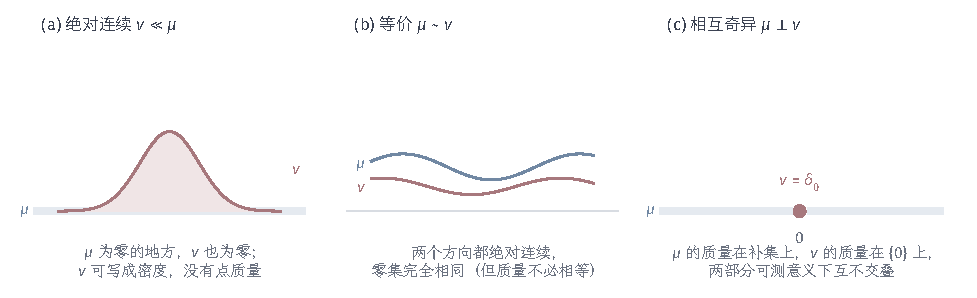
\includegraphics[width=169mm]{figures/01-mathematical-preliminaries-upper/04-space-and-geometry/02-measure-spaces/tikz/zero-set-relations/figure.pdf}
\caption{同一参考测度（蓝色横线）下，两种测度之间的三种零集关系。(a) 绝对连续$\nu\ll\mu$：$\nu$（红色密度）只在$\mu$有质量的地方取非零值，没有点质量。(b) 等价$\mu\sim\nu$：两个方向都绝对连续，零集完全相同，但同一区域上的质量大小仍可不同。(c) 相互奇异$\mu\perp\nu$：长度与点质量$\delta_0$各占一个可测范围，在可测意义下互不交叠。}
\label{fig:zero-set-relations}
\end{figure*}

\subsection{相对密度与测度分解}

本小节回答四个递进的问题：在什么条件下能找到密度、密度上的数值到底代表什么、怎样用它改写积分、以及当整个测度不能由密度表示时怎样把它拆开。
需要强调，这里的“导数”$d\nu/d\mu$是\emph{两种积分权重之比}，与坐标对坐标的普通导数没有关系。

\subsubsection{相对密度的存在与几乎处处唯一}

\paragraph{相对密度的存在与有限性}

绝对连续只告诉我们零集相容，我们还希望更具体：用一个函数$f$就能恢复$\nu$在\emph{每一个}可测集上的质量。

\begin{theorem}[Radon–Nikodym定理]
\label{thm:measure-radon-nikodym}
设$\mu,\nu$是同一可测空间上的非负$\sigma$有限测度，且$\nu\ll\mu$。
则存在非负可测函数$f$，使
\[
 \nu(A)=\int_A f\,d\mu\qquad(A\in\mathcal A).
\]
\end{theorem}

这个$f$记作$\dfrac{d\nu}{d\mu}$，称为$\nu$相对于$\mu$的\term{Radon–Nikodym密度}。
它的直觉是：在$x$附近取一个很小的可测块，$\nu$给这块的质量约等于$f(x)$乘以$\mu$给它的质量，密度就是两种称重方式在局部的换算比例。
$\sigma$有限是本定理常用的充分条件，不应说成一切密度存在的必要条件；对已经写出连续密度或离散权重的情形，那个已知函数本身就是Radon–Nikodym密度。

目标测度$\nu$的$\sigma$有限性还能保证密度不取无穷值。
设$E_k$覆盖$X$且$\nu(E_k)<\infty$，考虑$N=\{f=\infty\}$：
若$\mu(N\cap E_k)>0$，则$\nu(E_k)=\int_{E_k}f\,d\mu\geq+\infty$，矛盾。
故每个$N\cap E_k$都是$\mu$零集，可数并得$\mu(N)=0$。
因此总可以选一个几乎处处有限的代表，这也为后面等价测度取倒数做了准备。

\paragraph{密度的几乎处处唯一}

密度只在“零测集可以忽略”的意义下唯一。
若$f,g$都恢复$\nu$，把空间切成有限质量块、再把函数取值切成有界层和严格间隔层，就能在每一块上比较。
关键一步是：在某个$f\geq g+1/m$的可测层$D$上，两种表示给出
\[
 \int_Df\,d\mu=\nu(D)=\int_Dg\,d\mu,
\]
但若$\mu(D)>0$，左侧至少比右侧多$\mu(D)/m>0$，矛盾，所以$D$是零集。
可数合并所有块、所有层，得到$f>g$和$g>f$的集合都是零集，即
\[
 \frac{d\nu}{d\mu}=f=g\qquad\mu\text{几乎处处}.
\]
在$\mu$零集上随意改动密度值不影响任何集合的测度，所以密度并不规定每一个点上的数值，只规定“几乎处处”的局部比例。

\subsubsection{密度值与单点质量}

\paragraph{密度系数与单点质量的区别}

密度描述的是质量\emph{怎样沿集合分布}，不是“某一点上的概率”，这两者很容易混淆。
若$\nu=f\mu$且$\{x\}$可测，则
\[
 \nu(\{x\})=\int_{\{x\}}f\,d\mu.
\]
等式两边是不同对象：右边是用密度系数在单点上累计出的质量。

在$[0,1]$上取概率密度$p(x)=1$和$q(x)=2x$。
两者给每个单点的质量都是零，但在区间$[0,1/2]$上的质量不同：
\[
 \int_0^{1/2}1\,dx=\frac12,\qquad
 \int_0^{1/2}2x\,dx=\frac14.
\]
可见密度值大并不代表该点概率大，密度控制的是一整段区域的质量。

只有当参考测度在单点上本身有正质量，即$0<\mu(\{x\})<\infty$时，单点上的积分才退化为乘法$f(x)\mu(\{x\})$，此时
\[
 f(x)=\frac{\nu(\{x\})}{\mu(\{x\})}
\]
才真正是两点质量之比——离散权重表中的相对频率正是这种情形。
反过来，若$\mu(\{x\})=0$，随便改$f(x)$都不会改变测度。

用$\delta_0$还能看清密度表示的边界：任何普通非负函数$f$在单点$\{0\}$上的勒贝格积分都是$0$，不可能恢复$\delta_0(\{0\})=1$，所以$\delta_0$没有相对勒贝格测度的普通密度。
广义函数里的Dirac-$\delta$要在分布理论中另立框架，不能当成Radon–Nikodym可测函数；同理，也不能指望“在某个点填一个无穷大密度值”就表示出点质量。

\subsubsection{积分的换测度公式}

\paragraph{用相对密度改写积分}

有了密度$f=d\nu/d\mu$，对$g$的积分就能换一种参考测度来算：
\[
 \int_X g\,d\nu=\int_X gf\,d\mu.
\]
这个等式先对指示函数$g=\mathbf 1_A$成立（它就是Radon–Nikodym表示本身），再对简单函数由线性成立，最后对一般非负可测$g$由单调逼近成立，允许两边同为$+\infty$。
它做的事情只是“换一杆秤来称同一个函数”，输入点没有移动，输出集合也没有重新生成。
对有符号$g$则分别处理正负部分，在不会出现$+\infty-(+\infty)$时合并；特别地
\[
 \int|g|\,d\nu=\int|g|f\,d\mu
\]
把两种写法下的绝对可积条件对齐。

\paragraph{重加权、限制与归一化}

换测度公式反过来用就是“造一个新测度”：取非负可测权重$w$，定义
\[
 \nu(A)=\int_Aw\,d\mu.
\]
可数可加性由指标上的可加性和单调收敛保证。
若总权重$Z=\int_Xw\,d\mu$满足$0<Z<\infty$，归一化后$Q(A)=\nu(A)/Z$就是概率测度，密度为$w/Z$；$Z=0$或$Z=+\infty$时无法这样归一化。

取$w=\mathbf 1_E$得到\term{限制测度}$\mu_E(A)=\mu(A\cap E)$，归一化后就是“只在$E$内部按原相对比例分配质量”的条件分布。
注意三种“限制”的区别：乘以权重改变的是赋权、底集不变；推前测度会把输入点送到另一个空间；限制到子$\sigma$代数则只是减少可见集合。
在$[0,1]$均匀概率下取$w=2\mathbf 1_{[0,1/2]}$，得到的概率把全部质量放在前半段，它对原测度绝对连续，却不再等价——原来有质量的后半段被压成了零。

\paragraph{链式换参考与倒数公式}

密度可以像换算单位一样连乘。
若$\rho\ll\nu\ll\mu$，对集合指标连续换两次参考，得到链式法则
\[
 \frac{d\rho}{d\mu}=\frac{d\rho}{d\nu}\frac{d\nu}{d\mu}
 \qquad\mu\text{几乎处处},
\]
在密度为零处把乘积约定为零，避免无意义的$0\cdot\infty$。

如果两测度等价$\mu\sim\nu$，密度$f=d\nu/d\mu$不仅几乎处处非零，还几乎处处有限，于是可以取倒数。
对可测集$B$，
\[
 \int_B\frac1f\,d\nu=\int_B\frac1f\,f\,d\mu=\mu(B),
\]
所以$d\mu/d\nu=1/f$在$\nu$几乎处处成立。
单向绝对连续不足以走到这一步——密度可能在一整块区域上为零，倒数会爆炸。
用常数权重检验方向最直观：$\nu=2\mu$、$\rho=3\nu$时，$d\nu/d\mu=2$、$d\rho/d\nu=3$、$d\rho/d\mu=6$，反向$d\mu/d\nu=1/2$。
这些公式的依据始终是“恢复所有可测集上的质量”，不能形式地把微分符号当分数约掉。

\subsubsection{Lebesgue分解}

\paragraph{绝对连续部分与奇异部分}

拿一杆参考秤$\mu$去称一个新测度$\nu$，最理想的情况是处处都有换算密度。
但现实中$\nu$可能是两笔性质完全不同的“钱”：一笔均匀摊开、能用面积密度按平方计费，另一笔却集中放在个别点上、只按个数收固定费用。
拿面积秤去称第二笔，读数恒为零，怎么乘密度都乘不出那笔固定费用。
最典型的例子就是
\[
 \nu=\lambda+\delta_0,
\]
它给开区间$(a,b)$（不含$0$）的读数是长度$b-a$，却给单点$\{0\}$读数$1$。
所以整体地问“$\nu$有没有密度”会得到尴尬答案：它一部分能写成密度、另一部分写不成。

Lebesgue分解的作用，就是把这两笔账干净地分开：

\begin{theorem}[Lebesgue分解]
\label{thm:measure-lebesgue-decomposition}
设$\mu,\nu$是同一可测空间上的非负$\sigma$有限测度。
则存在唯一的非负测度$\nu_{\mathrm{ac}},\nu_{\mathrm s}$，使
\[
 \nu=\nu_{\mathrm{ac}}+\nu_{\mathrm s},\qquad
 \nu_{\mathrm{ac}}\ll\mu,\qquad
 \nu_{\mathrm s}\perp\mu.
\]
\end{theorem}

绝对连续部分再用Radon–Nikodym定理写成$\nu_{\mathrm{ac}}=f\mu$，于是每个集合的质量都拆成两笔：
\[
 \nu(A)=\int_Af\,d\mu+\nu_{\mathrm s}(A).
\]
两个定理的分工要分清：Lebesgue分解负责把“能连续表示的”和“必须单独放的”分开，Radon–Nikodym只负责表示其中的第一部分。
当奇异部分非零时，$f$不能称为整个$\nu$的密度。

\begin{figure*}[htbp]
\centering
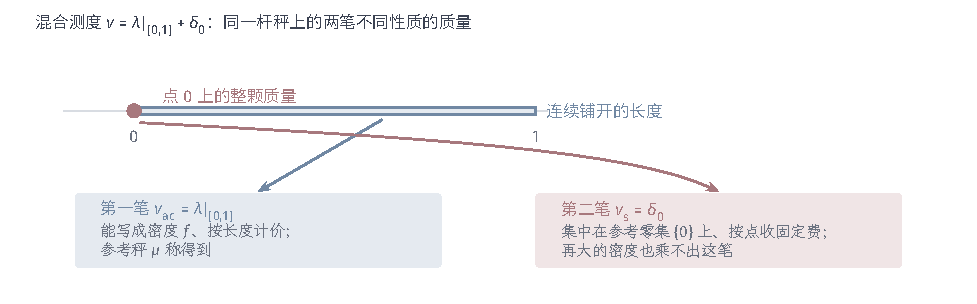
\includegraphics[width=169mm]{figures/01-mathematical-preliminaries-upper/04-space-and-geometry/02-measure-spaces/tikz/lebesgue-decomposition/figure.pdf}
\caption{Lebesgue分解像把混合收入拆成两笔计价规则不同的账。$\nu=\lambda|_{[0,1]}+\delta_0$中，连续铺开的长度$\nu_{\mathrm{ac}}$可以写成密度、按长度计价，参考测度$\mu$称得到；集中在参考零集$\{0\}$上的点质量$\nu_{\mathrm s}$按点收固定费，任何普通密度都乘不出这笔。每个集合收到的总质量等于两笔之和。}
\label{fig:lebesgue-decomposition}
\end{figure*}

\paragraph{分解的示例与参考测度依赖}

再看$[0,1]$上参考$\mu=\lambda|_{[0,1]}$、$\nu=\lambda|_{[0,1]}+\delta_0$这个例子，两部分的归属一目了然：铺在区间上的长度对$\mu$绝对连续（按面积的那笔），点$0$上的质量与$\mu$奇异（固定费那笔），所以
\[
 \nu_{\mathrm{ac}}=\lambda|_{[0,1]},\qquad \nu_{\mathrm s}=\delta_0.
\]
不含$0$的区间只收到长度$b-a$，集合$\{0\}$只收到点质量$1$，含$0$的区间则两笔都要算。

更通俗地说，Lebesgue分解有点像会计把一笔混合收入拆成“按面积结算”和“按点结算”两张单子：只要报上来的还是同一空间的集合，两张单子合起来就是总收入，可两张单子的计价规则谁也代替不了谁。

哪张单子非空，取决于你选用哪杆参考秤，所以分解是相对于所选参考而言的，不是测度自带的标签。
同一个$\nu$，若改取参考$\mu'=\nu$，那么每一笔质量都能按“自己称自己”换算，密度恒为$1$、奇异部分为零。
还要再次强调：奇异部分不必是孤立点；在更一般的例子里它可以由不可数个点组成、自身完全连续，却整体铺在一个参考零集上（例如后面会遇到的Cantor集）。

\subsection{有限有符号测度与全变差}

要量化两个非负测度的差异，最直接的想法是逐集合相减。
但相减的结果允许为负，不再是测度；我们需要先弄清这种“带符号的集合赋权”具有什么结构，它的正负部分和绝对变化总量怎样定义，然后才能用它给出概率之间的\term{全变差距离}。

\subsubsection{有限有符号测度与\term{总变差测度}}
\label{sec:measure-signed-total-variation}

\paragraph{集合赋权的正负分量}

对两个有限非负测度，定义
\[
 \eta(A)=\mu(A)-\nu(A).
\]
它仍然可数可加，但$\eta(A)$可以是负数。
这种取有限实值、可数可加的集合赋权称为有限\term{有符号测度}。
请注意区分：这里允许取负值的是\emph{给集合的赋权本身}，与“函数有正有负、但积分测度仍非负”是两回事。

\begin{theorem}[\term{Hahn分解}与\term{Jordan分解}]
\label{thm:measure-hahn-jordan}
对有限有符号测度$\eta$，存在互不相交且并为$X$的可测集$E_+,E_-$，使$\eta$在$E_+$的每个可测子集上非负、在$E_-$的每个可测子集上非正。
令
\[
 \eta^+(A)=\eta(A\cap E_+),\qquad
 \eta^-(A)=-\eta(A\cap E_-),
\]
则$\eta^+,\eta^-$是相互奇异的非负有限测度，且
\[
 \eta=\eta^+-\eta^-;
\]
这两个Jordan分量作为测度是唯一的。
\end{theorem}

Hahn分解选出的正负区域可以不唯一，但由此得到的正、负分量测度唯一。
可以用一张“结账表”来想这件事：同一批事件上，有的项目要额外收费（正分量）、有的项目给退款（负分量），Jordan分解就是把这张表拆成“收费单”和“退款单”两张分别只含正数的单子；总营业额是两单之差，账面上净收$0$只说明两单金额相等，绝不等于什么都没发生。
例如$\eta=\delta_0-\delta_1$在$\{0\}$上为$+1$、在$\{1\}$上为$-1$，全空间总和为$0$，可这个“总和为零”绝不意味着$\eta$处处为零。
也请把Jordan分解与Lebesgue分解区分开：前者按\emph{正负号}拆分一张有收有退的账单，后者按\emph{按面积还是按点计费}拆分一笔非负收入，两种拆分服务于不同问题。

\paragraph{总变差测度与有符号积分}

把正负部分重新加起来，得到总变差测度和\term{总变差范数}：
\[
 |\eta|=\eta^++\eta^-,\qquad
 \|\eta\|_{\mathrm{var}}=|\eta|(X).
\]
对集合$A$的任意有限分割，各块绝对赋权之和不超过$|\eta|(A)$，而按$A\cap E_+$、$A\cap E_-$分割恰好取等号；因此$|\eta|(A)$也是“把$A$切成任意小块后，绝对质量总和”的最大值。
它的作用是累计正负变化、不让它们抵消：$\eta(X)=0$时总变差仍可能很大。

对满足$\int|g|\,d|\eta|<\infty$的可测函数，定义对有符号测度的积分
\[
 \int g\,d\eta=\int g\,d\eta^+-\int g\,d\eta^-,
\]
于是
\[
 \left|\int g\,d\eta\right|\leq\int|g|\,d|\eta|
 \leq\|g\|_\infty\|\eta\|_{\mathrm{var}}.
\]
这说明要控制一个有符号赋权的积分读数，必须看它的总变差，不能只看可能正负抵消的净值$\eta(X)$。
特别地，若$\eta(A)=\int_Af\,d\mu$且$f$可积，则$f^+\mu$和$f^-\mu$正是它的Jordan分量，故$|\eta|=|f|\mu$，这把有符号测度又接回了熟悉的非负积分。

\subsubsection{全变差距离与测试积分}

现在专门比较两个概率测度$P,Q$。
先引入一个共同参考会很方便：令$\lambda=P+Q$。
因为$P,Q$都是有限测度且都对$\lambda$绝对连续，由Radon–Nikodym定理可写
\[
 p=\frac{dP}{d\lambda},\qquad q=\frac{dQ}{d\lambda}.
\]
在这个共同参考下，两者密度之差$p-q$的正负部分恰好等重——这会带来全变差特有的$1/2$系数。

\paragraph{事件质量差与密度公式}

最直接的比较，是看两个概率在同一个事件上的读数最多差多少：
\[
 \operatorname{TV}(P,Q)=\sup_{A\in\mathcal A}|P(A)-Q(A)|.
\]
它只关心“同一事件、两种权重”，不涉及事件在空间中的位置。
由概率质量介于$0,1$之间可知$0\leq\operatorname{TV}\leq1$；对称性、三角不等式和“距离为零即两测度相同”都可直接验证，所以TV是概率测度间的真正距离。

为什么它又等于密度差的$L^1$距离的一半？令$h=p-q$。
因为总质量都是$1$，$\int h\,d\lambda=0$，$h$的正部总量等于负部总量。
取正差集合$A_+=\{p\geq q\}$，任何事件上的质量差都不超过正部总量，而$A_+$恰好达到它；正负两部分合在一起得
\[
 \operatorname{TV}(P,Q)
 =\frac12\int|p-q|\,d\lambda
 =\frac12|P-Q|(X).
\]
$1/2$来自两个概率总质量相等（正差、负差各算一次才是$\int|p-q|$）；换成另一个共同有限参考，事件差上确界不变，所以数值与参考选择无关。
但若比较的是总质量不等的一般有限测度，这个$1/2$约定就要重新考虑。

\paragraph{有界观测量的误差控制}

TV之所以有用，是因为它立刻控制有界函数的期望误差。
若$g$取值在$[a,b]$内，先减去常数$(a+b)/2$再用密度差估计：
\[
 \left|\int g\,dP-\int g\,dQ\right|
 \leq(b-a)\operatorname{TV}(P,Q).
\]
特别地，$0\leq g\leq1$时系数为$1$，而正差集合的示性函数正好达到上确界，所以
\[
 \operatorname{TV}(P,Q)=\sup_{0\leq g\leq1}\left|\int g\,dP-\int g\,dQ\right|.
\]
若改用归一化$\|g\|_\infty\leq1$，系数则为$2$。
这两个“测试函数”表示后面比较测度核时还会用到。
几何上，TV只认事件不认位置：$a\neq b$时$\operatorname{TV}(\delta_a,\delta_b)=1$，无论两点离得近还是远；这个缺口正是\term{Wasserstein距离}要补的。

\subsection{\term{Hellinger距离}与KL散度}

全变差累计的是密度的绝对差$|p-q|$。
同样在共同参考下比较密度，还可以换成别的函数：对平方根差累计得到Hellinger距离，对有向对数比求期望得到KL散度。
它们衡量的是密度差异的不同侧面，因此性质也不同。

\subsubsection{Hellinger距离}

\paragraph{平方根密度与参考无关性}

定义
\[
 H^2(P,Q)=\frac12\int(\sqrt p-\sqrt q)^2\,d\lambda,
\qquad H(P,Q)=\sqrt{H^2(P,Q)}.
\]
用$\int p=\int q=1$展开，可化成更便于计算的形式
\[
 H^2(P,Q)=1-\int\sqrt{pq}\,d\lambda.
\]
其中$\int\sqrt{pq}$是密度的“几何平均重叠”，由Cauchy–Schwarz不等式介于$0,1$之间，所以$0\leq H\leq1$。
$H$只在$P,Q$共享的质量区域上统计重叠，与共同参考的选择无关。

\paragraph{距离性质与端点情形}

非负性、对称性显然；$H=0$等价于$\sqrt p=\sqrt q$几乎处处，即两概率相同。
三角不等式可在三者统一参考$P+Q+R$下，对平方根差用Cauchy–Schwarz证明。
两个端点也很直观：$P=Q$时$H=0$；$P\perp Q$时两者正密度区域不相交、$\sqrt{pq}=0$，$H=1$。
请注意距离是开平方后的$H$，不是$H^2$。

\subsubsection{KL散度与有限性}

\paragraph{有向定义与积分合法性}

\term{KL散度}衡量“用$Q$的编码去描述$P$时平均多花多少信息量”，它是\emph{有方向}的。
当$P\ll Q$时，定义
\[
 D_{\mathrm{KL}}(P\|Q)=\int\log\frac{dP}{dQ}\,dP
 =\int p\log\frac pq\,d\lambda,
\]
用自然对数；若$P$不对$Q$绝对连续（$Q$为零处$P$却有正质量），约定$D_{\mathrm{KL}}=+\infty$。

这个积分总是有良好定义的。写成$f=dP/dQ$后被积函数是$f\log f$；由$t\log t\geq-1/e$，其负部被$Q(X)=1$控制，不会出现$-\infty$，正部则允许为$+\infty$。
非负性来自$t\log t\geq t-1$：
\[
 D_{\mathrm{KL}}(P\|Q)=\int f\log f\,dQ\geq\int(f-1)\,dQ=0,
\]
等号只在$f=1$即$P=Q$时成立。
一定要把“积分有定义”和“积分有限”分开：绝对连续只保证前者，不保证后者。

\paragraph{方向差别与无穷值的例子}

交换$P,Q$会同时改变加权测度和对数比，所以两个方向的KL一般不同，它既不对称也不满足三角不等式，不能当距离用。
两点概率$P=(1/2,1/2)$、$Q=(3/4,1/4)$就能算出两个不同的有限值。

更能说明问题的是“互相绝对连续但KL无穷”。
在正整数上取重尾分布$p_n=c/n^2$和几何分布$q_n=(e-1)e^{-n}$：每个点两者权重都为正，零集关系完全相容；但
\[
 \log\frac{p_n}{q_n}=n-2\log n+O(1),
\]
在大$n$处$p_n\log(p_n/q_n)$像$1/n$一样衰减，其和发散。
可见“存在密度”只解决零集问题，对数比是否有足够的可积性是另一项独立要求。

\subsubsection{全变差、Hellinger与KL的关系}
\label{sec:measure-metric-relations}

固定同一对概率，三种指标可以在一定程度上互相控制。

\paragraph{全变差与Hellinger的双向控制}

由$(\sqrt a-\sqrt b)^2\leq|a-b|$积分，得
\[
 H^2(P,Q)\leq\operatorname{TV}(P,Q).
\]
反方向把$|p-q|=|\sqrt p-\sqrt q|(\sqrt p+\sqrt q)$拆开并用Cauchy–Schwarz，结合$\operatorname{TV}=\frac12\int|p-q|$，得
\[
 \operatorname{TV}(P,Q)\leq\sqrt2\,H(P,Q).
\]
所以$H$趋零和TV趋零是等价的，只是数值尺度不同。

\paragraph{Pinsker界与反向控制的边界}

自然对数下有\term{Pinsker不等式}
\[
 \operatorname{TV}(P,Q)^2\leq\frac12D_{\mathrm{KL}}(P\|Q).
\]
直觉是：KL在全部取值上的“信息差”，至少不小于只问“落在$P$更重的那一半没有”这个二元问题的信息差；对二元KL用凸性和二阶导数下界即可得到该式。
它的实用方向是：KL小就能推出TV小，进而控制所有事件概率和有界函数的期望差。

反方向一般不成立。取
\[
 P_\varepsilon=(1-\varepsilon)\delta_0+\varepsilon\delta_1,\qquad Q=\delta_0,
\]
则$\operatorname{TV}(P_\varepsilon,Q)=\varepsilon$可以任意小，但$P_\varepsilon$在$Q$的零集$\{1\}$上有正质量，$D_{\mathrm{KL}}(P_\varepsilon\|Q)=+\infty$。
所以一串分布在TV下逼近，KL却可能始终无穷。

\subsection{共同底层距离下的Wasserstein比较}

TV、Hellinger、KL都只在固定位置上比较密度或事件，完全不使用“两点相隔多远”的信息：$\delta_a$与$\delta_b$只要$a\neq b$，TV就是$1$。
本小节加上空间自带的距离$d$，让“把质量从一处搬到另一处要走多远”也进入差异的度量。

\subsubsection{\term{耦合}与质量配对}

\paragraph{两个边缘与耦合候选}

固定同一度量空间$X$上的概率$P,Q$。
一个耦合就是乘积空间$X\times X$上的联合概率$\gamma$，它的两个边缘恰好是$P,Q$：
\[
 \gamma(A\times X)=P(A),\qquad
 \gamma(X\times B)=Q(B).
\]
满足这两条边缘约束的全体联合概率记为$\Pi(P,Q)$。
可以把$\gamma$想象成一张“运输方案”：$\gamma(A\times B)$表示从源区域$A$搬到目标区域$B$的质量份额，行方向保证源质量不增不减，列方向保证目标收到恰好的质量。
耦合不一定来自一个确定映射——同一源点的质量允许拆给多个目标点；独立耦合$P\otimes Q$总是可行，说明候选集合非空。

\subsubsection{Wasserstein距离}

\paragraph{距离幂成本与有限矩范围}

给定完备可分度量$d$和$1\leq p<\infty$，先把讨论限制在$p$阶矩有限的概率上：固定基点$x_0$，令
\[
 \mathcal P_p(X)=\left\{P:\int d(x,x_0)^p\,dP(x)<\infty\right\}.
\]
换基点不改变这个集合，因为到两个基点的距离只相差常数倍。

对$P,Q\in\mathcal P_p(X)$，在所有运输方案中最小化总搬运代价，再开$p$次方恢复距离尺度：
\[
 W_p(P,Q)=\left(\inf_{\gamma\in\Pi(P,Q)}
 \int d(x,y)^p\,d\gamma(x,y)\right)^{1/p}.
\]
距离$d$衡量位置差，边缘约束保证质量守恒。
有限代价的候选确实存在：对独立耦合用不等式
\[
 d(x,y)^p\leq2^{p-1}\bigl[d(x,x_0)^p+d(y,x_0)^p\bigr],
\]
右边由两者的有限$p$阶矩控制。
但“候选非空”“最优代价有限”“最小值被某个耦合取到”是三个不同结论，后者要靠紧性，不能从下确界自动得到。

\paragraph{距离性质与最优计划的范围}

在Polish空间和有限矩条件下，$W_p$是$\mathcal P_p(X)$上的真正距离，且最优耦合存在：三角不等式要把两份耦合在中间空间拼接，同一性说明零成本只能在对角线上配对，存在性则依赖耦合族的紧性（\ref{sec:measure-tightness}小节会证明）。
最优耦合不一定由确定性映射实现；矩不足时代价可为无穷；没有共同距离时更无法定义$W_p$。

\paragraph{点质量与有限分布的计算}

两个点质量之间只有一种配对，所以
\[
 W_p(\delta_a,\delta_b)=d(a,b):
\]
全部质量从$a$搬到$b$，代价就是两点距离。
这与TV形成鲜明对照——后者恒为$1$，前者随两点接近而趋于零。
对有限离散分布$P=\sum_i\alpha_i\delta_{x_i}$、$Q=\sum_j\beta_j\delta_{y_j}$，求$W_p$就是在线性约束
\[
 \gamma_{ij}\geq0,\qquad
 \sum_j\gamma_{ij}=\alpha_i,\qquad
 \sum_i\gamma_{ij}=\beta_j
\]
下最小化$\sum_{i,j}\gamma_{ij}d(x_i,y_j)^p$，这正是经典的离散运输问题；产品耦合给出可行点，有限维紧可行集保证最小值取到。

\subsection{测试函数族与比较方式的对照}

各种距离到底控制了什么？一个统一的看法是：把每个函数看成一次“观测”或“探针”，两种测度在允许的探针上的积分读数最多差多少，就决定了差异能在多大程度上被观测到。

\subsubsection{指定观测类的最大积分差}

\paragraph{允许的观测与可辨认范围}

给定一类实值可测函数$\mathcal F$，定义
\[
 d_{\mathcal F}(P,Q)
 =\sup_{f\in\mathcal F}\left|\int f\,dP-\int f\,dQ\right|,
\]
称为\term{积分概率度量}。
它遍历的是“允许读取的观测”，不是源点也不是耦合。
如果观测类太小，它可能分不开不同测度：取$P=\frac12\delta_{-1}+\frac12\delta_1$、$Q=\delta_0$，只用$f(x)=x$探测时两边均值都是$0$，差异完全看不见。
函数类允许放大的倍数也必须受限，否则一个非零积分差乘任意大常数会使上确界成为无穷。
前面的TV正是这种观点的两个特例：用$0\leq f\leq1$的探针得到TV，用$\|f\|_\infty\leq1$的探针得到$2\operatorname{TV}$。

\subsubsection{Lipschitz观测与一阶Wasserstein}

\paragraph{由耦合成本控制积分差}

若探针$g$是$L$-Lipschitz函数，它对位置小幅移动不敏感，敏感性被$L$控制。
对任意耦合$\gamma$，把积分差写成联合形式：
\[
 \int g\,dP-\int g\,dQ
 =\int[g(x)-g(y)]\,d\gamma(x,y).
\]
由$|g(x)-g(y)|\leq L\,d(x,y)$，
\[
 \left|\int g\,dP-\int g\,dQ\right|
 \leq L\int d(x,y)\,d\gamma.
\]
对所有耦合取下确界，得到
\[
 \left|\int g\,dP-\int g\,dQ\right|\leq L\,W_1(P,Q).
\]
这给出一个非常实用的解释：$W_1$小，意味着任何对位置小幅移动不敏感的观测，其期望误差都小。
这里只证明了一个方向。

\paragraph{Lipschitz测试的对偶表示}

事实上反方向也成立，这就是\term{Kantorovich–Rubinstein对偶}：
\[
 W_1(P,Q)
 =\sup_{\operatorname{Lip}(f)\leq1,\ f(x_0)=0}
 \left|\int f\,dP-\int f\,dQ\right|.
\]
总质量相等允许给$f$减去任意常数（不改变积分差），基点归零后函数增长完全由距离控制。
反向等号是标准的对偶结论，不是前面那一行不等式能推出来的，但它说明$W_1$恰好等于“最敏感的1-Lipschitz探针”看到的差异。

\subsubsection{权重差异与位置差异的对照}

用点质量把几类指标并排放在一起最能说明问题。对$a\neq b$：
\[
 \operatorname{TV}(\delta_a,\delta_b)=1,\quad
 H(\delta_a,\delta_b)=1,\quad
 D_{\mathrm{KL}}(\delta_a\|\delta_b)=+\infty,
\]
而
\[
 W_p(\delta_a,\delta_b)=|a-b|.
\]
前三者只问“事件或密度是否相同”，只要不是同一个点就判为完全不同；Wasserstein还问“隔得多远”，$b$越接近$a$差异越小。
所以关心有界观测误差时用TV/Hellinger/KL，允许小范围搬动质量时用Wasserstein，两类问题不能互相替代。

再看有限离散分布与连续分布：有限支撑的点概率$\widehat P$和无原子概率$P$相互奇异，TV恒为$1$，无论点取多密都不能在TV下逼近连续目标；要谈粒子近似是否有效，必须改用弱观测或几何标准并附加抽样条件。
至此，同一空间上的比较工具已经齐备；下一节让输入和输出位于不同空间，研究质量怎样在空间之间传递。

\section{不同空间上的映射与比较}
\label{sec:measure-cross-space}

上一节的两种测度始终生活在同一个空间里，可以直接比较同一个事件。
但在机器学习中，输入和输出往往是不同性质的对象：图片与类别、状态与动作、一句外语与一句母语。
这时要先解决“质量怎样从一个空间传到另一个空间”，才能谈比较。

本节沿三条递进的线索展开。
第一条是\emph{确定映射}：每个输入被送到唯一的输出点，输入测度由此在输出空间诱导出一个\term{推前测度}。
第二条把确定映射放宽为\term{测度核}：每个输入不再对应一个点，而是对应输出空间上的一项概率分布——这正是“随机通道”“转移概率”的抽象。
第三条保留输入与输出的配对信息，用\emph{联合测度}同时描述两边，并研究何时能从联合分布反推出条件核；最后再讨论给定跨空间成本时的最优运输。
请始终注意：输出端是否匹配、以及实现这种匹配要搬动多远，是两个不同的问题。

\subsection{\term{可测映射}的推前与密度变换}

\subsubsection{\term{推前测度}与输出积分}

\paragraph{推前的定义与质量边界}

设$T:(X,\mathcal A)\to(Y,\mathcal B)$是一个可测映射，$\mu$是输入空间上的测度。
对任意目标集合$B$，一个很自然的问题是：$T$把多少输入质量送进了$B$？
答案就是$B$的原像上的输入质量：
\[
 (T_\#\mu)(B)=\mu\bigl(T^{-1}(B)\bigr).
\]
这样定义的$T_\#\mu$称为推前测度（也叫像测度）。
可测性在这里的作用是保证$T^{-1}(B)$一定是输入端的合法可测集；记号$T^{-1}$只表示取原像，并不要求$T$可逆。

$T_\#\mu$确实是一个测度：空集的原像为空，质量为零；不相交集合的原像仍不相交，且取原像与可数并可交换，所以可数可加性从$\mu$原样传过来。
又因为$T^{-1}(Y)=X$，总质量守恒：
\[
 (T_\#\mu)(Y)=\mu(X).
\]
因此有限测度推前后仍有限，概率推前后仍是概率。
但$\sigma$有限不一定保持：实轴上无限的勒贝格测度被常值映射$T(x)=0$压到一个点上，得到总质量为$+\infty$的$\delta_0$，输出空间再也无法被有限质量集覆盖。
若多个源点映到同一目标点，该点收到的质量就是各源点权重之和。

\paragraph{输出观测在输入端的表示}

推前测度最重要的计算性质，是把“对输出的平均”翻译成“对输入的平均”。
先在指示函数$g=\mathbf 1_B$上看：
\[
 \int_Y\mathbf 1_B\,d(T_\#\mu)
 =(T_\#\mu)(B)=\mu(T^{-1}B)
 =\int_X\mathbf 1_B(Tx)\,d\mu.
\]
经简单函数和非负单调逼近，对任意非负可测$g$都有
\begin{equation}
 \int_Y g\,d(T_\#\mu)=\int_X g(Tx)\,d\mu(x),
 \label{eq:measure-pushforward-integral}
\end{equation}
即“$g$在输出端的平均，等于$g\circ T$在输入端的平均”；有符号函数在绝对可积时同样成立。
这个恒等式是后面一切核计算和矩计算的入口。

接连使用两个映射时，先送$T$再送$S$与直接送复合映射一致：
\[
 (S\circ T)_\#\mu=S_\#(T_\#\mu),
\]
因为$(S\circ T)^{-1}(C)=T^{-1}(S^{-1}(C))$。
若某个自映射$T:X\to X$恰好满足$T_\#\mu=\mu$，称它\term{保持测度}，例如抛硬币中“交换正反面”的操作；这只是质量守恒的一个特例。

\subsubsection{输出密度与质量重组}

\paragraph{回用欧氏换元计算输出密度}

推前恒等式~\eqref{eq:measure-pushforward-integral}并不要求输出有密度；只有在给定参考体积且映射足够光滑时，才能谈输出密度长什么样。
设$U,V\subseteq\mathbb R^d$是同维开集，$T:U\to V$是$C^1$微分同胚（全局一一对应、逆映射光滑），输入测度相对勒贝格体积有密度$p$。
对非负测试函数$g$，先用推前恒等式，再用多元换元：
\[
 \int_Vg(y)\,d(T_\#\mu)(y)
 =\int_U g(Tx)\,p(x)\,dx
 =\int_V g(y)\,p(T^{-1}y)\,|\det DT^{-1}(y)|\,dy.
\]
对所有$g$都成立，所以输出密度为
\[
 q(y)=p(T^{-1}y)\,|\det DT^{-1}(y)|,
\]
等价地
\[
 q(Tx)\,|\det DT(x)|=p(x).
\]
直觉是：映射在$x$附近把体积放大了$|\det DT(x)|$倍，密度就要相应缩小同样倍数，才能保持小块质量不变。
平移只平移密度$q(y)=p(y-b)$；可逆线性映射$T(x)=Ax$给出$q(y)=p(A^{-1}y)/|\det A|$；镜像等负行列式映射由绝对值处理。
多对一、降维或退化映射不满足全局微分同胚条件，不能随便选一个逆分支套公式，必须老老实实用原像把所有分支的贡献加起来。

\paragraph{合并、投影与原子输出}

即使不可逆，推前测度仍然有定义，只是输出未必有普通密度。
两个典型情形值得对比。
一是投影：若$\mathbb R^2$上有密度$p(x,y)$，$T(x,y)=x$，则目标集合$B$的原像是$B\times\mathbb R$，由Tonelli定理
\[
 (T_\#\mu)(B)=\int_B\left(\int_{\mathbb R}p(x,y)\,dy\right)dx,
\]
所以输出仍是连续分布，边缘密度是把被积掉的坐标积分掉：$q(x)=\int p(x,y)\,dy$。
二是常值映射$T(x,y)=y_0$：任何目标集合的原像不是全空间就是空集，有限输入总质量$m$被整个压成一个原子$m\delta_{y_0}$，在正维空间里相对勒贝格测度没有普通密度。
对比可见：不可逆映射既可能输出连续密度，也可能输出原子；而“一个输入只对应一个输出点”始终是确定映射的限制。
若同一个输入还要按随机性把质量分给多个输出，就需要下一小节的测度核。

\subsection{测度核与\term{测度值映射}}

\subsubsection{随输入变化的输出权重}

\paragraph{测度核的两项条件}

先用有限情形建立直觉。
设输入、输出都是有限集合，一个“随机转移规则”就是一张非负矩阵$K$：第$x$行第$y$列的数表示输入$x$把多少质量送给输出$y$，把一行中若干列加起来，就得到输入$x$送给某个输出集合的总质量。
把这个想法搬到一般空间，会遇到两个要求：固定输入时，输出端的赋值必须是一个测度（才能对集合相加）；固定输出集合时，其质量随输入的变化必须可测（才能对输入测度积分）。

\begin{definition}[测度核]
\label{def:measure-kernel}
设$(X,\mathcal A)$、$(Y,\mathcal B)$是可测空间。映射
\[
 K:X\times\mathcal B\to[0,\infty]
\]
若满足：
\begin{enumerate}
 \item 对每个$x\in X$，$K_x=K(x,\cdot)$是$(Y,\mathcal B)$上的非负测度；
 \item 对每个$B\in\mathcal B$，函数$x\mapsto K(x,B)$是$\mathcal A$可测函数，
\end{enumerate}
就称$K$为从$X$到$Y$的\term{测度核}，记作$K:X\leadsto Y$。
\end{definition}

第一条管“每个输入怎样在输出端分配质量”，第二条管“这种分配怎样随输入可测地变化”，缺一不可。
请注意这里的测度核与函数空间章里衡量相似度的正定核（kernel function）只是同名，数学对象完全不同。

一般定义不限制每个$x$送出多少总质量。
本章的运算为方便起见，额外假设存在一个与$x$无关的$M<\infty$，使
\[
 K(x,Y)\leq M\qquad\text{对所有 }x,
\]
称为统一有限质量界；逐点有限$K(x,Y)<\infty$并不等于有共同上界。
若进一步
\[
 K(x,Y)=1\qquad\text{对所有 }x,
\]
则称$K$为\term{归一化测度核}（概率核、马尔可夫核）：无论输入是什么，送出的总质量恰好为$1$。
归一化是额外条件，不写进一般核的定义。

确定映射是核的最简单特例。
对可测映射$T:X\to Y$，取
\[
 K_T(x,B)=\delta_{T(x)}(B)=\mathbf 1_B(Tx):
\]
每个输入把全部质量集中在唯一输出点$T(x)$，它是一个归一化核。
所以“推前”只是“核传递”当每行都是点质量时的特例；一般核允许输入把质量分散到多个输出，且总质量可以随输入变化。

\begin{figure*}[htbp]
\centering
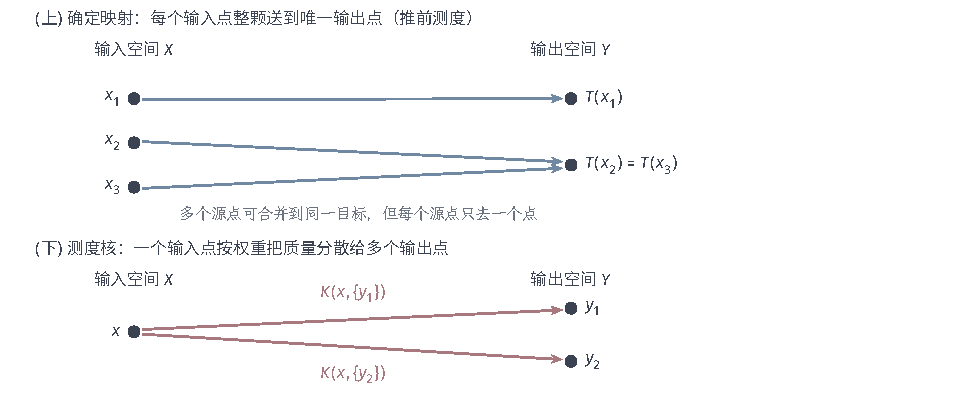
\includegraphics[width=169mm]{figures/01-mathematical-preliminaries-upper/04-space-and-geometry/02-measure-spaces/tikz/pushforward-and-kernel/figure.pdf}
\caption{确定映射（推前测度）与测度核的对照。上排：每个输入点的全部质量沿唯一箭头送到一个输出点，多个输入点可以合并到同一目标（$x_2,x_3$），但单个输入点不能拆开。下排：一般测度核允许同一个输入$x$按权重$K(x,\{y_1\})$、$K(x,\{y_2\})$把质量分给多个输出；归一化核满足这些权重之和为$1$。}
\label{fig:pushforward-and-kernel}
\end{figure*}

\subsubsection{核积分与核复合}

\paragraph{输出测度与观测函数的传递}

有了输入测度$\mu$和核$K$，怎样得到输出空间上的总测度？
直观上是“每个输入$x$送出质量分布$K_x$，再按$\mu$中$x$的权重把这些分布加权求和”：
\[
 (\mu K)(B)=\int_X K(x,B)\,\mu(dx).
\]
对固定$x$，$K(x,\cdot)$可数可加；对不相交的$B_n$，用单调收敛把求和与积分交换，可知$\mu K$仍是测度。
其总质量为
\[
 (\mu K)(Y)=\int_XK(x,Y)\,d\mu\leq M\mu(X).
\]
因此统一质量界保证有限输入测度产生有限输出测度；核归一化时总质量守恒$(\mu K)(Y)=\mu(X)$，一般核则不守恒。

对应地，输出函数$g$沿核传回输入：
\[
 Kg(x)=\int_Y g(y)\,K(x,dy).
\]
对非负可测$g$，$Kg$可测，并且有核积分恒等式
\begin{equation}
 \int_Y g\,d(\mu K)=\int_X Kg\,d\mu,
 \label{eq:measure-kernel-integral}
\end{equation}
即“先核传递再对输出取平均”等于“先沿核算条件平均、再对输入平均”。
有界函数满足$|Kg(x)|\leq M\|g\|_\infty$；一般有符号函数在绝对可积时可选取可测版本后合并。

用一个小数字例子核对。
输入点$a,b$的质量分别为$1,2$，输出点$0,1$；核的两行取$(2,1)$和$(0,2)$（注意这不是归一化核）。
输出两点的质量分别是
\[
 1\cdot2+2\cdot0=2,\qquad 1\cdot1+2\cdot2=5,
\]
总质量$7$等于按输入权重累计的行总质量$1\cdot3+2\cdot2=7$，但不等于输入总质量$3$。
取$g(y)=y$，沿核的条件平均在两行是$1,2$，输入加权$1\cdot1+2\cdot2=5$，与直接对输出积分一致。

\paragraph{连续两次传递的复合}

若$K:X\leadsto Y$、$L:Y\leadsto Z$，从$X$经$Y$到$Z$的总规则是“先按$K_x$在$Y$中取一个中间点，再按该点的$L$核送出”，即
\[
 (KL)(x,C)=\int_Y L(y,C)\,K(x,dy).
\]
统一质量界相乘：$(KL)(x,Z)\leq N\,K(x,Y)\leq NM$；两核都归一化时复合核也归一化。
先后传递与先后传回观测彼此一致：
\[
 (\mu K)L=\mu(KL),\qquad (KL)g=K(Lg).
\]
把$K,L$取成映射$T,S$的点核，就恢复$K_TK_S=K_{S\circ T}$，说明核复合是映射复合的自然推广。

\subsubsection{测度值映射的可测性}

\paragraph{用集合质量检验测度族的可测依赖}

有时要把“一个$X$上的点映到$Y$上的一整项测度”本身看成映射$F:X\to\mathcal M_+(Y)$。
怎样定义这种映射可测？
在测度空间$\mathcal M_+(Y)$上，用所有评价映射
\[
 e_B(\nu)=\nu(B),\qquad B\in\mathcal B
\]
生成一个$\sigma$代数。
在这个结构下，$F$可测当且仅当对每个$B$，$x\mapsto F(x)(B)$都是可测函数——也就是说，\emph{每个目标集合收到的质量随输入可测地变化}。
测度核的第二条条件恰好保证$x\mapsto K_x$是这样一项可测的测度值映射。

一个直接的例子是经验测度：给定非负权重$a_i$，
\[
 F(y_1,\ldots,y_n)=\sum_{i=1}^n a_i\delta_{y_i}
\]
对每个$B$的评价$\sum_i a_i\mathbf 1_B(y_i)$都是坐标的可测函数，所以“由样本点形成加权点测度”这个操作是可测的；取$a_i=1/n$就是常用的\term{经验测度}。

\subsection{联合测度与测度\term{核分解}}

输出测度$\mu K$只告诉我们目标端最终收到多少质量，却丢掉了“哪部分输入送给了哪部分输出”的配对信息。
要保留这种信息，必须在乘积空间$X\times Y$上使用联合测度。
本小节先正向构造联合测度，再研究反向问题：给定一个联合测度，能否恢复“给定输入时输出的条件分布”。

\subsubsection{由输入测度和核构造联合测度}

\paragraph{联合权重、两个边缘与乘积特例}

给定有限输入测度$\mu$和核$K:X\leadsto Y$，先在矩形上规定
\[
 J(A\times B)=\int_A K(x,B)\,\mu(dx),
\]
含义是“从$A$中的输入出发、最终落入$B$的质量”。
再推广到一般乘积可测集：
\[
 J(E)=\int_X\left[\int_Y\mathbf 1_E(x,y)\,K(x,dy)\right]\mu(dx).
\]
截面积分关于$x$可测，单调收敛保证$J$可数可加，总质量不超过$M\mu(X)$。

在矩形上取$B=Y$和$A=X$，得到两个边缘：
\[
 (\pi_X)_\#J(A)=\int_A K(x,Y)\,d\mu(x),\qquad
 (\pi_Y)_\#J=\mu K.
\]
第一边缘是“每个输入实际送出多少质量”，只有核归一化时它才等于原$\mu$；第二边缘就是前面的输出测度。
对联合函数$h$，相应积分规则为
\begin{equation}
 \int_{X\times Y}h\,dJ
 =\int_X\int_Y h(x,y)\,K(x,dy)\,\mu(dx),
 \label{eq:measure-joint-integral}
\end{equation}
记号$\mu(dx)K(x,dy)$表示的就是这种“先输入、再沿条件核”的联合累计。

两个特例帮助定位。
若$K(x,\cdot)=\nu$与$x$无关，$J$就是乘积测度$\mu\otimes\nu$（“输入与输出独立地各算各的”）。
若$K=K_T$是确定映射的点核，$J=(\operatorname{id},T)_\#\mu$是集中在图像$\{(x,Tx)\}$上的\term{图测度}（“输出完全由输入确定”）。
乘积和图测度都只是联合测度的特例；给定同样的边缘，通常还有许多携带不同配对信息的联合测度。

\subsubsection{从联合测度反求测度核}

\paragraph{子$\sigma$代数上的\term{条件积分}与观测值表示}

反向分解的核心问题是：只看输入$x$，输出$y$的条件分布是什么？
为理解它，先看一个预备概念——在较粗的信息下保留积分。
在有限测度空间上，给定可积函数$h$和子$\sigma$代数$\mathcal G$，把$\nu(A)=\int_Ah\,d\mu$限制到$\mathcal G$的集合上。
这个受限赋权对$\mu|_{\mathcal G}$绝对连续，由Radon–Nikodym定理存在$\mathcal G$可测的函数$H$，使
\[
 \int_A H\,d\mu=\int_A h\,d\mu\qquad(A\in\mathcal G).
\]
$H$就是$h$在“只能看到$\mathcal G$”时的积分代表：它保存每个粗集合上的累计，却不必逐点等于$h$。
这正是条件期望/条件积分的思想，这里只用它作为分解的桥梁。

若$\mathcal G=\sigma(S)$由某个观测$S$生成，则$H$只通过$S$取值：$H=\phi\circ S$。
也就是说，只能根据观测$S$得到的信息，必然是观测值的函数，而不能在“$S$相同、但不可区分”的点上给出不同值。

把这一想法用于联合测度$J$：令第一坐标投影为$\pi_X$、$\mathcal G=\sigma(\pi_X)$，对每个目标集$B$取$h=\mathbf 1_B(y)$。
条件积分只依赖$x$，记为$k_B(x)$，则
\[
 \int_A k_B(x)\,d\mu_X(x)=J(A\times B),
\]
其中$\mu_X=(\pi_X)_\#J$是第一边缘。
$k_B(x)$正是“给定输入$x$时输出落入$B$的条件概率”的雏形，取值在$[0,1]$。
但对每个$B$分别找到$k_B$，还不能保证它们彼此拼得起来：对固定的$x$，要求$B\mapsto k_B(x)$可加、且$k_Y(x)=1$；而逐集合用Radon–Nikodym定理得到的代表，可能在不同集合上各自挑了一个零测集上的取值，彼此冲突。
在有限情形里这毫无问题——条件分布就是联合频数表里每一行归一化：行内各列频数除以行和，天然加起来等于$1$。
一般空间的困难只在于“行”可以有不可数个、没有一张写好的频数表，需要下面的存在定理保证能选出一套彼此一致的行分布。

\paragraph{标准Borel范围内的联合分解}

\term{核分解}（条件分布的正则化）在足够规整的可测空间中一定存在。

\begin{theorem}[测度的核分解]
\label{thm:measure-disintegration}
设$X,Y$为标准Borel空间，$J$是$X\times Y$上的非零有限测度，第一边缘$\mu_X=(\pi_X)_\#J$。
则存在归一化测度核$K:X\leadsto Y$，使
\[
 J(A\times B)=\int_A K(x,B)\,\mu_X(dx),
\]
即
\[
 J=\mu_X(dx)\,K(x,dy),
\]
且第二边缘为$\mu_XK$。
\end{theorem}

直觉上，联合测度总能解释成“先按$\mu_X$抽取输入$x$，再按条件核$K_x$抽取输出$y$”；归一化是按实际第一边缘分解的结果，并不要求$J$本身是概率。
标准Borel空间的规整之处，是它的可测集合能由可数个基本集合决定，于是前面逐个集合得到的条件概率可以改造成一套彼此相容的行分布（这叫“正则版本”）；每个$x$送出的那一项$K_x$只在$\mu_X$的一个零集之外唯一——也就是说，对输入中几乎必然取到的点，条件分布没有歧义，个别零测输入点上怎样指定都不影响计算。

对角图测度的例子很能说明“联合密度”和“条件核”的区别。
令$X=Y=[0,1]$，$J=(\operatorname{id},\operatorname{id})_\#\lambda$集中在对角线$\{x=y\}$上。
它的两个边缘都是$\lambda$，但$\lambda\otimes\lambda$给对角线质量$0$、$J$给它质量$1$，所以$J$相对乘积测度没有密度；尽管如此，条件核$K(x,\cdot)=\delta_x$仍然把$J$完整重建。
因此“没有联合密度”和“没有条件分解”是两回事。

\subsection{建立共同空间后的测度比较}

有了推前和核，就能把位于不同空间的测度“搬到同一个地方”再用上一节的指标比较。
本小节强调：比较的对象是变换后的输出，比较结果只反映这种特定表示能看到的差异；表示本身可能丢失信息。

\subsubsection{目标空间与共同表示}

\paragraph{指定映射后的目标端差异}

给定输入空间上的概率$P$、目标空间上的概率$Q$和固定映射$T:X\to Y$，先形成$R=T_\#P$，再在$Y$上比较$R$与$Q$。
我们不能直接对不同空间的$P,Q$做密度相减，因为同一个目标事件$B$对应的其实是源事件$T^{-1}(B)$。
用核时同理，取$R=PK$；一般核可能改变总质量，比较前要先核对输出范围。

各类指标需要的条件照旧：TV、Hellinger只需在$Y$上取共同有限参考$R+Q$；$D_{\mathrm{KL}}(R\|Q)$要检查$R\ll Q$和对数可积性；Wasserstein则要求$(Y,d_Y)$是Polish空间且$R,Q$有有限$p$阶矩。
尤其要注意：输出矩要在输出空间计算，
\[
 \int d_Y(y,y_0)^p\,dR(y)=\int d_Y(Tx,y_0)^p\,dP(x),
\]
源空间的矩不能代替它。
例如输入是$[0,1]$上的均匀分布、$T(x)=1/x$（$x>0$），输入各阶矩都有限，但输出矩$\int_0^1x^{-p}dx=+\infty$，输出分布无法进入Wasserstein的有限距离范围。

\paragraph{在共同表示空间中比较}

若两侧都要换表示，就固定映射$S:X\to Z$、$T:Y\to Z$，在第三个空间$Z$上比较$S_\#P$与$T_\#Q$。
比较什么指标，就在$Z$上配什么结构：比权重差异取共同参考，比几何差异则让$Z$成为Polish度量空间并核对矩，再算$W_p^Z(S_\#P,T_\#Q)$。
$X,Y$内部各自的距离$d_X,d_Y$并不能自动给出一个跨空间距离$d(x,y)$。
这种比较的结果依赖所选表示：若把两侧都映成同一个常值，输出当然完全相同，却只说明该常值表示看不到任何输入差异，不能说明原对象相同。

\subsubsection{输出规则与可辨认范围}

\paragraph{确定映射下的信息丢失}

取$P_1=\delta_{-1}$、$P_2=\delta_1$和绝对值映射$T(x)=|x|$：两个截然不同的输入分布推前后都变成$\delta_1$，目标端TV、Hellinger、Wasserstein差异全部为零。
输出相同只意味着“用$|x|$这个观测分不开$+1$和$-1$”。

对同一个映射$T$，比较在变换后只会变小：逐事件有
\[
 |(T_\#P_1)(B)-(T_\#P_2)(B)|
 =|P_1(T^{-1}B)-P_2(T^{-1}B)|
 \leq\operatorname{TV}(P_1,P_2),
\]
取上确界得
\[
 \operatorname{TV}(T_\#P_1,T_\#P_2)\leq\operatorname{TV}(P_1,P_2).
\]
原因是输出端能检验的事件，只对应输入端的一部分事件（原像）。
但两侧用的是\emph{不同}表示时，这个收缩不成立：同为$\delta_0$的输入，经$S(0)=0$和$T(0)=1)$后输出TV为$1$。

\paragraph{同一归一化测度核下的TV控制}

固定同一个归一化核$K$，输出差为
\[
 |(PK)(B)-(QK)(B)|
 =\left|\int_XK(x,B)\,d(P-Q)(x)\right|.
\]
由于$0\leq K(x,B)\leq1$，利用TV的$[0,1]$测试表示，每个事件差不超过$\operatorname{TV}(P,Q)$，故
\[
 \operatorname{TV}(PK,QK)\leq\operatorname{TV}(P,Q).
\]
同一个随机通道不会增大可区分性，这就是“数据处理”在TV下的形式。
条件是同一核且归一化：核不同、或核不归一化（总质量改变）时结论不适用。

\paragraph{共同输入构造耦合上界}

若两个输出来自同一个带随机性的源，可用一个共同空间上的映射$F,G$构造它们的耦合$\gamma=(F,G)_\#R$，其两边缘为$F_\#R,G_\#R$。
当两输出在同一Polish空间且矩有限时，
\[
 W_p^p(F_\#R,G_\#R)
 \leq\int d(F(\omega),G(\omega))^p\,dR(\omega).
\]
应用中共同源可以是“共享噪声”：用同一个随机种子驱动两个随机系统，输出差异可用输入空间中$F,G$的距离上界控制。
这只给出一个可行耦合的成本上界，不一定最优。

\subsection{给定跨空间成本的运输比较}

到目前为止，比较要么发生在同一空间，要么先经表示映到同一空间。
但有时源空间$X$和目标空间$Y$天然不同，我们想直接问：把$X$上的质量改造成$Y$上的质量，最少要付出多大代价？
这时必须由问题本身给定一份跨空间成本表，数学不会自动从两个内部距离造出它。

\subsubsection{乘积空间上的耦合与成本}

\paragraph{跨空间质量匹配与成本累计}

把耦合推广到$X\times Y$：$\Pi(P,Q)$是所有满足
\[
 \gamma(A\times Y)=P(A),\qquad \gamma(X\times B)=Q(B)
\]
的跨空间联合概率，两个边缘约束分别保证“源质量不增不减”和“目标收到恰好的量”。
再给定一个非负的、对乘积可测的成本函数$c:X\times Y\to[0,\infty]$，定义最优运输成本
\[
 \mathcal C_c(P,Q)
 =\inf_{\gamma\in\Pi(P,Q)}\int c(x,y)\,d\gamma(x,y).
\]
它在所有质量守恒的配对中找总代价最小的一个。

请注意$\mathcal C_c$一般不是距离：成本$c$未必对称，甚至两侧空间不同时无从谈对称；取$c\equiv0$会让任何$P,Q$的成本都是零。
只有当$X=Y$、取$c(x,y)=d(x,y)^p$且矩有限时，它才成为$W_p^p$。

\subsubsection{运输映射与\term{运输计划}}

\paragraph{不可拆分的映射与可拆分的计划}

历史上有两个版本的运输问题。
\term{Monge问题}要求每个源点的质量完整送到一个目标点，即在约束$T_\#P=Q$下最小化$\int c(x,T(x))\,dP$。
\term{Kantorovich问题}放松为允许拆分：在全部耦合$\gamma\in\Pi(P,Q)$中最小化$\int c\,d\gamma$。
在标准Borel空间，计划还可由核分解写成$P(dx)K(x,dy)$，其中$K$由第一边缘$P$分解故归一化，约束$PK=Q$表示每个源点送出的总质量为$1$、各目标收到的总量正确。

一个最小的例子说明放松拆分为什么必要。
源只有一个点$X=\{0\}$，目标有两个点$Y=\{-1,1\}$，$P=\delta_0$而$Q=\frac12\delta_{-1}+\frac12\delta_1$。
任何确定映射只能把唯一源点送到一个目标，Monge问题无解；但计划
\[
 \gamma=\tfrac12\delta_{(0,-1)}+\tfrac12\delta_{(0,1)}
\]
允许把源点的质量对半拆，满足全部约束。
反过来，任何可行映射$T$的图计划都是一个Kantorovich耦合，所以映射问题嵌入计划问题；计划可行不代表映射可行。

\subsubsection{成本判定与比较范围}

\paragraph{可行、有限与达到分别判断}

使用最优运输成本时要分三步检查，不能混为一谈。
第一，可行性：独立耦合$P\otimes Q$总在$\Pi(P,Q)$中，所以计划可行域非空（这与Monge问题可能无解形成对照）。
第二，有限性：要有至少一个有限成本的候选，例如$\int c\,d(P\otimes Q)<\infty$；若$c$处处为$+\infty$，最优值只能是无穷。
第三，达到性：最小值是否真的被某个耦合取到，还需紧性与成本的下半连续性；其证明要用到\ref{sec:measure-tightness}小节的一致紧性和下半连续积分界，这里先引用结论。

\paragraph{目标匹配、运输代价与结构比较边界}

最后用一个小例子把两类问题彻底分开。
取$X=\{a\}$、$Y=\{b\}$、$P=\delta_a$、$Q=\delta_b$、$T(a)=b$，并规定$c(a,b)=7$。
在输出端，$T_\#P=Q$，匹配得完美无缺，同空间差异为$0$；但实现这个匹配的唯一跨空间运输成本是$7$。
“是否得到了目标分布”和“得到它要花多大代价”显然是两个问题。
因此跨空间比较之前必须先明确给定的是映射、核、共同表示还是成本函数；仅凭两个空间各自的内部距离，本书并不推导空间之间的“内在结构距离”，那是更专门的理论。

\section{测度的收敛与极限操作}
\label{sec:measure-convergence}

有了比较两个概率分布的各种指标，自然要问：一整列分布$P_1,P_2,\ldots$什么时候算趋近于某个$P$？
这个问题没有唯一答案，因为“趋近”取决于我们用什么探针去观测。
本节按探针从强到弱排列几种收敛：要求每个事件的误差一致消失的全变差收敛、只要求有界连续观测收敛的弱收敛、再加上距离矩尾部控制的Wasserstein收敛。
然后建立弱收敛下三件常用的事——事件概率怎么读、连续变换是否保持收敛、无界成本的极限下界——并回答“一族分布是否总能挑出收敛子列”。
最后把序列换成随时间变化的测度曲线，提醒不同时间尺度上的极限不能混用。
本节的比较都在同一个固定空间进行；不同空间的对象要先按上一节映到共同空间。

\subsection{测度序列的收敛方式}
\label{sec:measure-sequence-convergence}

\subsubsection{\term{逐集收敛}与全变差收敛}

\paragraph{从比较误差定义趋近}

最强的常用要求是全变差收敛：
\[
 \operatorname{TV}(P_n,P)\to0.
\]
它的含义是：存在一个与事件无关的误差界（就是TV）趋于零，从而\emph{同时}控制所有可测事件。
由前面的不等式，TV收敛等价于Hellinger收敛；KL收敛通过Pinsker界足以推出TV收敛，但反过来不成立（回想$P_\varepsilon=(1-\varepsilon)\delta_0+\varepsilon\delta_1$与$\delta_0$）。

把要求放松一档得到逐集收敛：对每一个\emph{固定}的事件$A$，
\[
 P_n(A)\to P(A).
\]
两者的差别完全在量词上。逐集收敛时，给定精度后需要等多少项$N$可以随事件$A$而变——复杂事件可能要等很久；TV收敛则要求同一个$N$对所有事件一起生效。
因此TV收敛必然推出逐集收敛，反之不然。
不过逐集收敛已经足以控制任意固定的有界可测函数$g$：先用简单函数在$\|g\|_\infty$意义下一致逼近$g$，再利用概率总质量为$1$控制逼近误差，得到
\[
 \int g\,dP_n\to\int g\,dP.
\]

\subsubsection{\term{弱收敛}与连续测试}

\paragraph{弱收敛与位置移动}

再放松一档，连“每个事件”都不要求，只保留对连续观测量的控制。
称$P_n$弱收敛到$P$，记作$P_n\Rightarrow P$，若对每个有界连续函数$\varphi$都有
\[
 \int\varphi\,dP_n\to\int\varphi\,dP.
\]
为什么只用连续函数做探针？因为事件指示函数$\mathbf 1_A$在集合边界上通常是跳变的，分布质量在边界附近的微小挪动会让$P_n(A)$剧烈变化，却不会明显影响任何连续函数的平均。

标准例子正是“质量在位置上不断靠近”。
取
\[
 P_n=\delta_{1/n},\qquad P=\delta_0.
\]
对任意有界连续$\varphi$，积分就是函数值$\varphi(1/n)\to\varphi(0)$，所以$P_n\Rightarrow P$；但事件$\{0\}$的概率始终是$0$而不是$1$，TV距离也始终为$1$。
质量明明在几何上越来越接近，逐事件比较却认为毫无进展——这清楚说明收敛结论依赖于所选标准。

\subsubsection{Wasserstein收敛与矩条件}

\paragraph{弱趋近与距离尾部的共同控制}

弱收敛只管“局部、有界”的观测，不管远处的质量；\term{Wasserstein距离}则会为远距离移动付费。
在Polish空间上，对$P_n,P\in\mathcal P_p(X)$有标准判据
\begin{equation}
 W_p(P_n,P)\to0
 \quad\Longleftrightarrow\quad
 P_n\Rightarrow P
 \ \text{且}\
 \int d(x,x_0)^p\,dP_n\to\int d(x,x_0)^p\,dP.
 \label{eq:measure-wasserstein-criterion}
\end{equation}
——既要在所有有界连续探针上收敛，又要$p$阶矩收敛。
矩条件控制的是“远处的小质量”。
记$z(x)=d(x,x_0)^p$。
先只用弱收敛，把它截断成有界函数$\min(z,R)$，能推出积分在近处（离基点不超过$R$）收敛；真正的差别在截断之外的“尾部”$\int(z-R)_+\,dP_n$。
全矩收敛加上弱收敛，可以推出一个对所有$n$统一成立的尾部估计：先取一个足够大的$R$把\emph{极限测度}的尾部压到很小，再用弱收敛保证$n$足够大时$P_n$在“$R$以外”的概率也很小，两者合起来就把整列的尾部一起压住。
这正是“距离的$p$次方关于这列测度一致可积”的含义；仅有“每个$P_n$自己的矩有限”给不出这种一致性。

\paragraph{小概率远距离的反例}

“每项矩有限”为什么不够？看下面的序列：
\[
 P_n=(1-n^{-p})\delta_0+n^{-p}\delta_n,\qquad P=\delta_0.
\]
远端那一点的概率只有$n^{-p}$，对任意有界连续观测的贡献趋于零，故$P_n\Rightarrow P$；每一项的$p$阶矩也都有限。
但把远端质量搬回原点要走距离$n$，代价是
\[
 W_p(P_n,P)^p=n^{-p}\cdot n^p=1,
\]
永不趋于零。
这把两件事分得很清楚：远端质量的\emph{概率}可以很小，但乘上很大的\emph{距离}后总代价仍是常数；没有对尾部的共同控制，Wasserstein不会收敛。

\begin{figure*}[htbp]
\centering
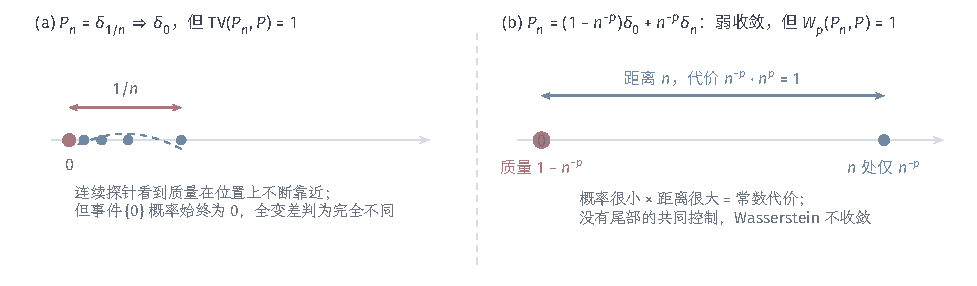
\includegraphics[width=169mm]{figures/01-mathematical-preliminaries-upper/04-space-and-geometry/02-measure-spaces/tikz/convergence-modes/figure.pdf}
\caption{两种“看起来在靠近、却不按更强标准收敛”的典型情形。(a) $P_n=\delta_{1/n}$在几何上不断靠近$\delta_0$，连续探针读数$\varphi(1/n)\to\varphi(0)$，故弱收敛；但事件$\{0\}$的概率始终为$0$，全变差距离恒为$1$。(b) $P_n=(1-n^{-p})\delta_0+n^{-p}\delta_n$弱收敛、每项矩都有限，但把$n$处那一点概率$n^{-p}$搬回原点的$p$次代价$n^{-p}\cdot n^p=1$，故$W_p$不趋于零。}
\label{fig:convergence-modes}
\end{figure*}

\subsection{弱收敛的判据与稳定性}

弱收敛只直接定义在有界连续测试上，实际使用时还想知道：事件概率能不能读、经过映射后还收不收敛、无界成本的极限保不保住下界。
这三者都是弱收敛这同一个概念下的推论，不是新的收敛方式。

\subsubsection{事件概率与边界质量}

弱收敛只在连续函数的积分上成立，可实际问题里我们常想直接读“落在某集合里的概率”。
什么时候这件事合法？答案是：只要极限分布不在该集合的\emph{边界}上放质量。
下面的\term{Portmanteau定理}先给出用开集、闭集表述的形式，事件概率的读法是它的直接推论：
\[
 P_n\Rightarrow P
\]
等价于对所有闭集$C$有$\limsup_nP_n(C)\leq P(C)$，也等价于对所有开集$G$有$\liminf_nP_n(G)\geq P(G)$。
用一句话说就是：当质量整体向$P$靠拢时，落在一个闭集里的概率最终不会超过$P$给它的概率（边界附近的质量可以溜出去），落在一个开集里的概率最终不会少于$P$给它的概率（质量可以从边界溜进来）。
它的实用推论是：如果极限测度不给集合$A$的边界质量，即$P(\partial A)=0$，那么
\[
 P_n(A)\to P(A).
\]

闭集方向可以直观地证明。对闭集$C$，用连续函数
\[
 h_k(x)=\max\{1-k\,d(x,C),0\}
\]
从外面“软包”一层：$h_k$有界连续、在$C$上等于$1$、离开$C$超过$1/k$就降到$0$，且$h_k\downarrow\mathbf 1_C$。
由$\mathbf 1_C\leq h_k$和弱收敛，
\[
 \limsup_nP_n(C)\leq\int h_k\,dP;
\]
再令$k\to\infty$，由支配收敛得到$\limsup_nP_n(C)\leq P(C)$。
开集方向取补集即可。
一般集合用内部$A^\circ$和闭包$\overline A$夹住：
\[
 P(A^\circ)\leq\liminf_nP_n(A)\leq\limsup_nP_n(A)\leq P(\overline A),
\]
只有边界质量为零时两端才相等。
回看$\delta_{1/n}$与事件$\{0\}$：极限测度恰好把质量放在边界$\{0\}$上，条件失败，所以$P_n(\{0\})$不收敛到$P(\{0\})$。
问题的根源始终是探针在集合边界上的跳变。

\subsubsection{连续推前与边缘保持}

弱收敛在连续变换下保持。
设$T:X\to Y$连续且$P_n\Rightarrow P$，对目标端任意有界连续$\varphi$，
\[
 \int\varphi\,d(T_\#P_n)=\int\varphi\circ T\,dP_n\to\int\varphi\circ T\,dP,
\]
因为$\varphi\circ T$仍有界连续。故
\[
 T_\#P_n\Rightarrow T_\#P.
\]
注意结论依赖\emph{连续性}：若$T$只可测不连续，可能失败。例如$P_n=\delta_{1/n}$、$P=\delta_0$，取$T=\mathbf 1_{\{0\}}$，则$T_\#P_n=\delta_0$而$T_\#P=\delta_1$。
连续坐标投影是这一结论的重要应用：若耦合列弱收敛，其两个边缘也分别弱收敛到极限耦合的边缘——这正是后面最优运输计划取极限时仍满足边缘约束的依据。

\subsubsection{\term{下半连续}成本的极限下界}

运输成本通常无界，不能直接当弱收敛的测试，但在下半连续时能保住一个方向的不等式。
所谓\term{下半连续}，直观上就是“极限点处的值不会突然变贵”：当$x_n\to x$时，恒有$c(x)\leq\liminf_n c(x_n)$——成本函数允许在某点向上跳变（如$c(x)=0$只在原点、其余为$1$），但不允许向下塌。
在这个条件下，非负下半连续函数$c$可以用一列有界连续函数从下方逼近：
\[
 c_k(x)=\min\left\{k,\ \inf_y[c(y)+k\,d(x,y)]\right\},
\]
$c_k$的$k$-Lipschitz连续性可直接验证，$c_k\uparrow c$则由下半连续性保证（若某点严格小于$c(x)$，近似取到的点必趋向$x$，与下半连续矛盾）。

设$P_n\Rightarrow P$。先固定$k$用弱收敛，再令$k\to\infty$用单调收敛：
\[
 \int c\,dP=\lim_k\int c_k\,dP
 =\lim_k\lim_n\int c_k\,dP_n
 \leq\liminf_n\int c\,dP_n.
\]
于是
\begin{equation}
 \int c\,dP\leq\liminf_n\int c\,dP_n.
 \label{eq:measure-lsc-portmanteau}
\end{equation}
直觉是：下半连续函数在“极限点处的值不超过附近点的下极限”，积分把这个性质继承下来；极限分布处的最优成本不会比逼近序列的成本下极限更贵。
这里测度本身在变，不能直接套用固定测度的Fatou引理。
这条不等式与紧性配合，正好证明最优运输计划可以取到。

\subsection{\term{一致紧性}与弱子列}
\label{sec:measure-tightness}

前面都是“先有候选极限$P$，再判断$P_n$是否趋近它”。
反过来的问题是：不给定极限，一列概率是否至少能挑出一个收敛子列？
在实轴上有界序列靠紧性总能取子列；一般空间中，类似结论成立的关键是“质量不能跑到任何紧集之外”。

\paragraph{一致紧性与极限子列}

称概率族$\mathcal F$一致紧，若对每个$\varepsilon>0$都能找到\emph{同一个}紧集$K_\varepsilon$，使族中每一个$P$都满足
\[
 P(X\setminus K_\varepsilon)<\varepsilon.
\]
紧集可以随精度$\varepsilon$变，但不能随具体的$P$变——要求的是“一整个族共用一个紧笼子”。
在一般度量空间中“有界”不一定“紧”，所以统一的矩界不能无条件代替一致紧性。

\begin{theorem}[\term{Prokhorov定理}，子列形式]
\label{thm:measure-prokhorov}
在Polish空间上，概率族$\mathcal F$一致紧，当且仅当$\mathcal F$中任意序列都有弱收敛到某个Borel概率的子列。
\end{theorem}

极限概率不必属于原来的族；“某种收敛如何定义”和“是否保证存在收敛子列”是两个独立判断。
质量逃逸的典型反例是$\{\delta_n:n\geq1\}$：每个$\delta_n$本身都是紧支撑的，但不存在一个能同时留住所有$n$的紧集，序列没有弱收敛到概率的子列。

\paragraph{固定边缘下的最优计划}

现在把紧性和下半连续界用到最优运输上，补齐“最优计划存在”的证明三步。
先证明\emph{整个}耦合族$\Pi(P,Q)$一致紧，而不只是某个耦合紧。
给定$\varepsilon>0$，用紧集$K,L$分别把$P,Q$的大部分质量套住：
\[
 P(K^c)<\frac\varepsilon2,\qquad Q(L^c)<\frac\varepsilon2.
\]
对任意$\gamma\in\Pi(P,Q)$，由边缘约束，
\[
 \gamma((K\times L)^c)\leq\gamma(K^c\times Y)+\gamma(X\times L^c)
 =P(K^c)+Q(L^c)<\varepsilon.
\]
于是所有耦合共用同一个紧集$K\times L$。

设成本$c$非负下半连续且至少有一个有限成本耦合，最优值
\[
 I=\inf_{\gamma\in\Pi(P,Q)}\int c\,d\gamma<\infty.
\]
取一列成本趋于$I$的耦合$\gamma_n$；由一致紧性和Prokhorov定理抽出弱收敛子列$\gamma_{n_k}\Rightarrow\gamma$。
连续投影保持边缘，所以$\gamma$仍是$P,Q$的耦合；下半连续积分界给出
\[
 \int c\,d\gamma\leq\liminf_k\int c\,d\gamma_{n_k}=I,
\]
而$\gamma$可行又给出反向不等式，故最小值在$\gamma$处达到。
这就把“紧子列—边缘保持—成本下界”三步接齐。
结论只保证最优\emph{计划}存在，不保证最优\emph{映射}存在；成本也必须下半连续。

\subsection{测度曲线与参数极限}

\paragraph{由序列判据读取时间连续性}

把序号$n$换成连续时间$t$，就得到概率曲线$t\mapsto\mu_t$。
称它弱连续，若每个有界连续探针的读数关于$t$连续，即
\[
 t_n\to t\ \Longrightarrow\ \mu_{t_n}\Rightarrow\mu_t.
\]
若各时刻都在$\mathcal P_p(X)$中，还可要求$W_p(\mu_{t_n},\mu_t)\to0$，由矩判据~\eqref{eq:measure-wasserstein-criterion}，这额外控制了尾部。

点质量曲线$\mu_t=\delta_t$再次显示标准的作用：
\[
 W_p(\mu_s,\mu_t)=|s-t|,
\]
所以它关于$W_p$连续；但$s\neq t$时TV恒为$1$，在全变差意义下处处不连续。
若不同时刻的测度位于不同空间，还要先固定到一个共同空间的表示，才能谈连续性。

\paragraph{固定时刻、有限时域与长时间}

比较一条近似曲线$\mu_t^h$与目标曲线$\mu_t$时，要区分三种越来越强的说法，它们的量词不能互换：
\begin{enumerate}
 \item \emph{固定时刻}：对每个固定$t$，$W_p(\mu_t^h,\mu_t)\to0$；
 \item \emph{有限时域一致}：对每个固定$T$，$\sup_{0\leq t\leq T}W_p(\mu_t^h,\mu_t)\to0$；
 \item \emph{长时间极限}：$t\to\infty$时曲线本身是否趋于某个极限。
\end{enumerate}
取$\mu_t=\delta_0$、$\mu_t^h=\delta_{ht}$（$h>0$）：固定$t$时误差为$ht\to0$，有限区间$[0,T]$上最大误差为$hT\to0$，但在随$h$移动的时刻$t=1/h$误差恒为$1$，所以在$t\geq0$全域上不一致收敛。
这提醒我们：数值近似在每个固定时刻、每个有限时间区间上可靠，并不自动推出长时间结论；演化方程、数值稳定性和极限交换都留给后续问题专门处理。


\FloatBarrier
\section{本章小结}

本章把微积分中“沿长度、体积累计”的想法推广到任意对象组成的空间，得到五条相互衔接的认识。

第一，测量分两层，而且两层互不相同。$\sigma$代数规定\emph{哪些集合看得见}，测度规定\emph{看得见的集合有多大}；还要把测度与度量分清：测度吃进一个集合给出份量，度量吃进两个点给出距离，同一底集上两者各自独立选择，讨论Wasserstein等几何问题时才在测度之外另加度量。同一个可测范围上可以配任意多种权重，也可以通过子$\sigma$代数在不删点的情况下降低分辨能力。有限、概率、$\sigma$有限是三种强度不同的质量条件，零测集和完备化说明哪些点上的例外可以忽略。当开集参与进来时，Borel结构、Polish空间和支持把“测量”与“位置”联系起来，而一般积分、三条收敛定理、乘积测度与Tonelli/Fubini都在明确条件下原样沿用。

第二，同一空间上的测度比较从零集关系开始，再到表示和定量指标。绝对连续、等价和相互奇异刻画零集之间的包含、重合与分离；Radon–Nikodym密度是两种称重方式的局部换算比例，Lebesgue分解把能这样换算的部分和集中在零集上的部分分开。为描述测度之差引入了有符号测度及其Jordan分解与总变差。全变差、Hellinger和KL只比较同一位置上的事件或密度，Wasserstein还要计入两点间的距离；积分概率度量把它们统一成“某类探针上的最大读数差”。这些指标回答的问题不同，不存在一个能代替其余的“万能距离”。

第三，跨空间时质量的传递规则从确定走向随机。可测映射的推前回答“每个输出事件收到多少输入质量”，输出积分等于输入上的复合积分；测度核把“一个输入对应一个点”放宽为“一个输入对应一项目标测度”，核积分和核复合分别统一了输出传递与观测传递。联合测度保留输入输出的配对，乘积和确定图是其特例；在标准Borel空间上，联合测度可以沿第一边缘分解为归一化条件核。条件积分只保存粗信息下的累计，条件期望等概率法则在后文展开。

第四，跨空间比较前必须先固定对应关系。给定映射或核以后，比较的是变换后的输出而不是原对象；表示可能丢失信息，所以输出相同不能反推输入相同，不同表示之间也没有收缩性质。给定跨空间成本时，Kantorovich计划允许拆分质量、Monge映射不允许，二者可行域不同；可行、有限、最优值达到要分别靠耦合非空、有限成本候选和紧性加下半连续性来保证。输出匹配为零与运输代价非零可以同时成立。

第五，测度序列是否趋近取决于探针。全变差统一控制所有事件，弱收敛只看有界连续函数，Wasserstein还要加上距离矩的尾部控制；弱收敛通过Portmanteau界读取边界零质量事件，在连续映射下保持，在下半连续成本下只给积分下界。一致紧性经Prokhorov定理保证弱子列，并支撑最优运输计划的存在性；固定时刻、有限时域一致和长时间极限是三种不能互换的逼近。
这些通用操作为后文的随机过程、条件模型、经验测度和策略分析提供了语言，但相应的概率性质、统计保证和生成机制仍需各自的条件。

